\chapter{Design} \label{section:design}
The design phase sets out to elaborate on the scenarios for experiments with IoT device. In these experiments, we compare and combine approaches from industry standards and papers presented in the analysis section. Conclusions are taken into consideration in establishing the plan of measurements and in the construction of the sensor unit.

\section{Research questions}
This thesis aims to provide answers to four research questions formulated in broader sense. The focus is primarily on making data flow more efficient in an industrial sensor network that monitors rotating machines. The \textbf{research questions} are:
\begin{enumerate}[label=RQ\arabic*., font=\bfseries]
    \itemsep0pt
	\item Which temporal and spectral features can be extracted from vibration signals to provide the most accurate record of machinery faults?
	\item What is the reduction in transmission goodput when chosen signal features are used?
	\item What accuracies of prediction models can be achieved with various feature subsets?
	\item How can machinery faults be continuously identified and predicted based upon collected events?
\end{enumerate}

\noindent In accomplishing the objectives of our research we propose several \textbf{goals}:
\begin{todolist}
    \itemsep0pt
	\item Statistically and visually describe vibration signals from the Machinery fault database (MauFaulDa).
	\item Establish a list of conditions that should be later investigated in the experimental setting.
	\item Prepare dataset to be used in conjunction with machine learning models, namely by identifying labels and balancing classes.
	\item Find the best subsets of features in temporal and spectral domain with previously analyzed feature extraction and selection methods.
	\item Evaluate the performance of models described in the diagnostics section with a significant focus on the k-nearest neighbor algorithm.
	\item Combine feature selection with online machine learning model.
	\item Acquire measurements of vibrations from machines in the real environment to form a novel dataset of machinery behavior.
	\item Develop hardware and implement its firmware to obtain such measurement in the quality demanded by vibrodiagnostics standards.
\end{todolist}

However, we leave out from our efforts experiments on the data features calculated from wavelets and peaks in the spectral domain. The reason is that we did not find a way to represent extracted features more succinctly as a single number. We also did not discover a strategy for choosing only the relevant frequency bins. The assembled description is retained to lead further research on that topic.

The goals are impacted by certain \textbf{risks} that are assessed and tracked:
\begin{enumerate}[label=R-\arabic*., font=\bfseries]
\itemsep0pt
\item Machines in the real environment will not be available for vibration measurements. \\ \emph{Mitigation}: Contact and establish collaboration with alternative partners. 
\item Repeated measurements will not be consistent, and a lack of data is obtained from different classes.
\\ \emph{Mitigation}: Prepare a plan for measurements and photo document sensor placements. 
\item Fault modes could not be reliably differentiated and labeled in the dataset.
\\ \emph{Mitigation}: Consult domain experts and machines' maintenance staff.
\item Suggestions made by exploring the MaFaulDa dataset will not be applicable in practice. \\
\emph{Mitigation}: When applicable, apply the same procedures as in MaFaulDa to measured data.
\end{enumerate}


\section{Dataset exploration}
In establishing the validity of methods to be deployed on the sensor node we explore the MaFaulDa dataset. It is the largest known machinery fault collection, so it is possible to create multiple subsets based on requested conditions. 

One representative recording is first selected in each available fault category. The sample is visualized and statistically described in both temporal and spectral domains. A whole step-by-step procedure is outlined in the activity diagram (Fig.~\ref{fig:design:mafaulda-preprocessing}).

\begin{figure}[ht]
	\centering
	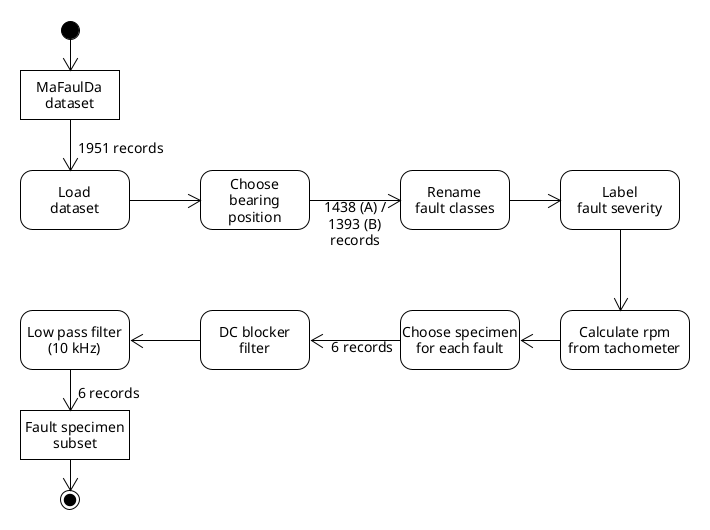
\includegraphics[width=\textwidth]{assets/design/activity-data-exploration.png}
	\caption{Activity diagram of MaFaulDa dataset preprocessing}
	\label{fig:design:mafaulda-preprocessing}
\end{figure}

MaFaulda contains 1951 records labeled with inducted faults of increasing severity. The defects were set up on the machine simulator as is mentioned in the part about datasets. Time series of the triaxial piezoelectric accelerometers in separate files have a sampling frequency of 50 kHz. 

These vibration sensors are placed in two positions. The first placement is around the inner underhang bearing named \emph{A} which is closer to the motor. The second location is around the outer overhang bearing denoted as \emph{B} position.

\subsection{Fault annotations}
The MaFaulDa has annotations altogether for 10 classes of faults of which there is 1 class for fault-free baseline operation, 3 classes for shaft defects, 3 classes for inner bearing defects, and 3 for outer bearing defects. Some categories are redundant or irrelevant for a given sensor position. 

Therefore rotor shaft misalignements in vertical and horizontal directions are merged into one joint group. Depending on the chosen bearing position only records having relevant labels are considered. 

This means that fault classification solely concerns bearing in the direct contact and shaft mechanically passing through it. The bearings affect each other, but the effect on the opposite side should appear via a common interconnection shaft. 

In the end, that leaves \textbf{6 types of labels}: baseline, two shaft faults are imbalance and misalignment, and three bearing faults are cage fault, ball fault, and outer race fault. In the step of choosing the accelerometer location records pointing to the other bearing as a source of the malfunction are discarded. Then the next action renames the labels to be better recognizable and unite the same phenomena.

Groups of identified machine defects are additionally characterized by altered masses attached or motor shaft displacement shifts. The set amount is sorted in ascending order separating \textbf{multiple event severities}. However, the count of severity levels is not identical in every group. Levels are hence scaled into the range between zero and one using a min-max scaler. Scaling is applied to classes separately.

The strength of the recorded response by the underlying defect is also dependent on the shaft \textbf{rotational speed}. Speed in rpm is calculated from pulsed speedometer output. It is the average distance between two successive rising edges: 
\begin{ceqn}\begin{align}
\mathrm{rpm} = 60 \;/\; \overline{\Delta t}
\end{align}\end{ceqn}

\textbf{One specimen waveform} is picked from each fault class to illustrate their superficial differences. Recordings are filtered to get the highest severity levels and around a mean rotation speed of 2500 rpm (42 Hz)  to see the patterns most pronounced. The baseline class sample is chosen according to fixed rotor speed.


\subsection{Signal filters}
The DC component in the three-dimensional vibration signal is removed by subtracting the global mean. Immediately follows a digital IIR Butterworth \textbf{low pass filter} of \nth{5} order with cutoff frequency 10 kHz at -3 dB. 

Before the low pass filter usage, the peak at 20 kHz with sideband was present as an unwanted artifact. It could not have been reliably recorded due to the linear frequency response of the sensor up to 10 kHz. At the same time, such frequency is outside the range of any feasible MEMS accelerometer.

\begin{figure}[ht]
    \centering
    \begin{subfigure}[b]{0.44\textwidth}
        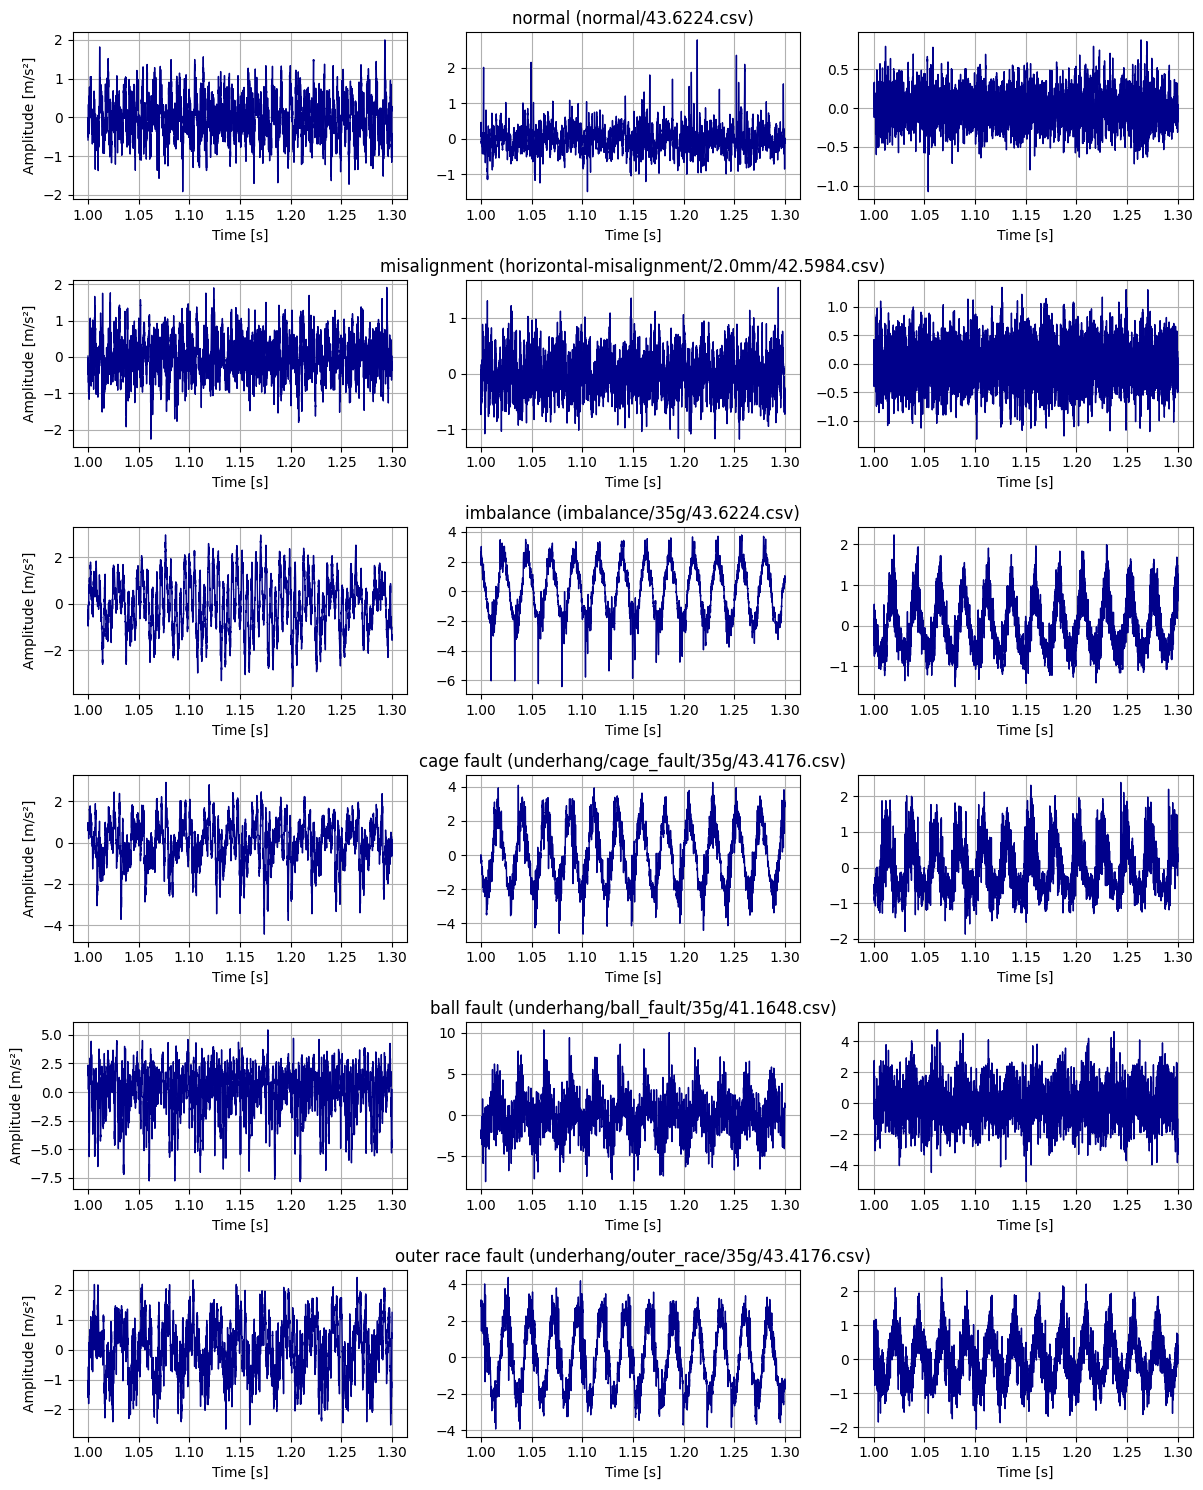
\includegraphics[width=\textwidth]{assets/design/Mafaulda-A-time-waveform.png}
        \caption{Temporal domain waveforms}
        \label{fig:design:fault-temporal-waveform}
    \end{subfigure}
    \hfill
    \begin{subfigure}[b]{0.55\textwidth}
        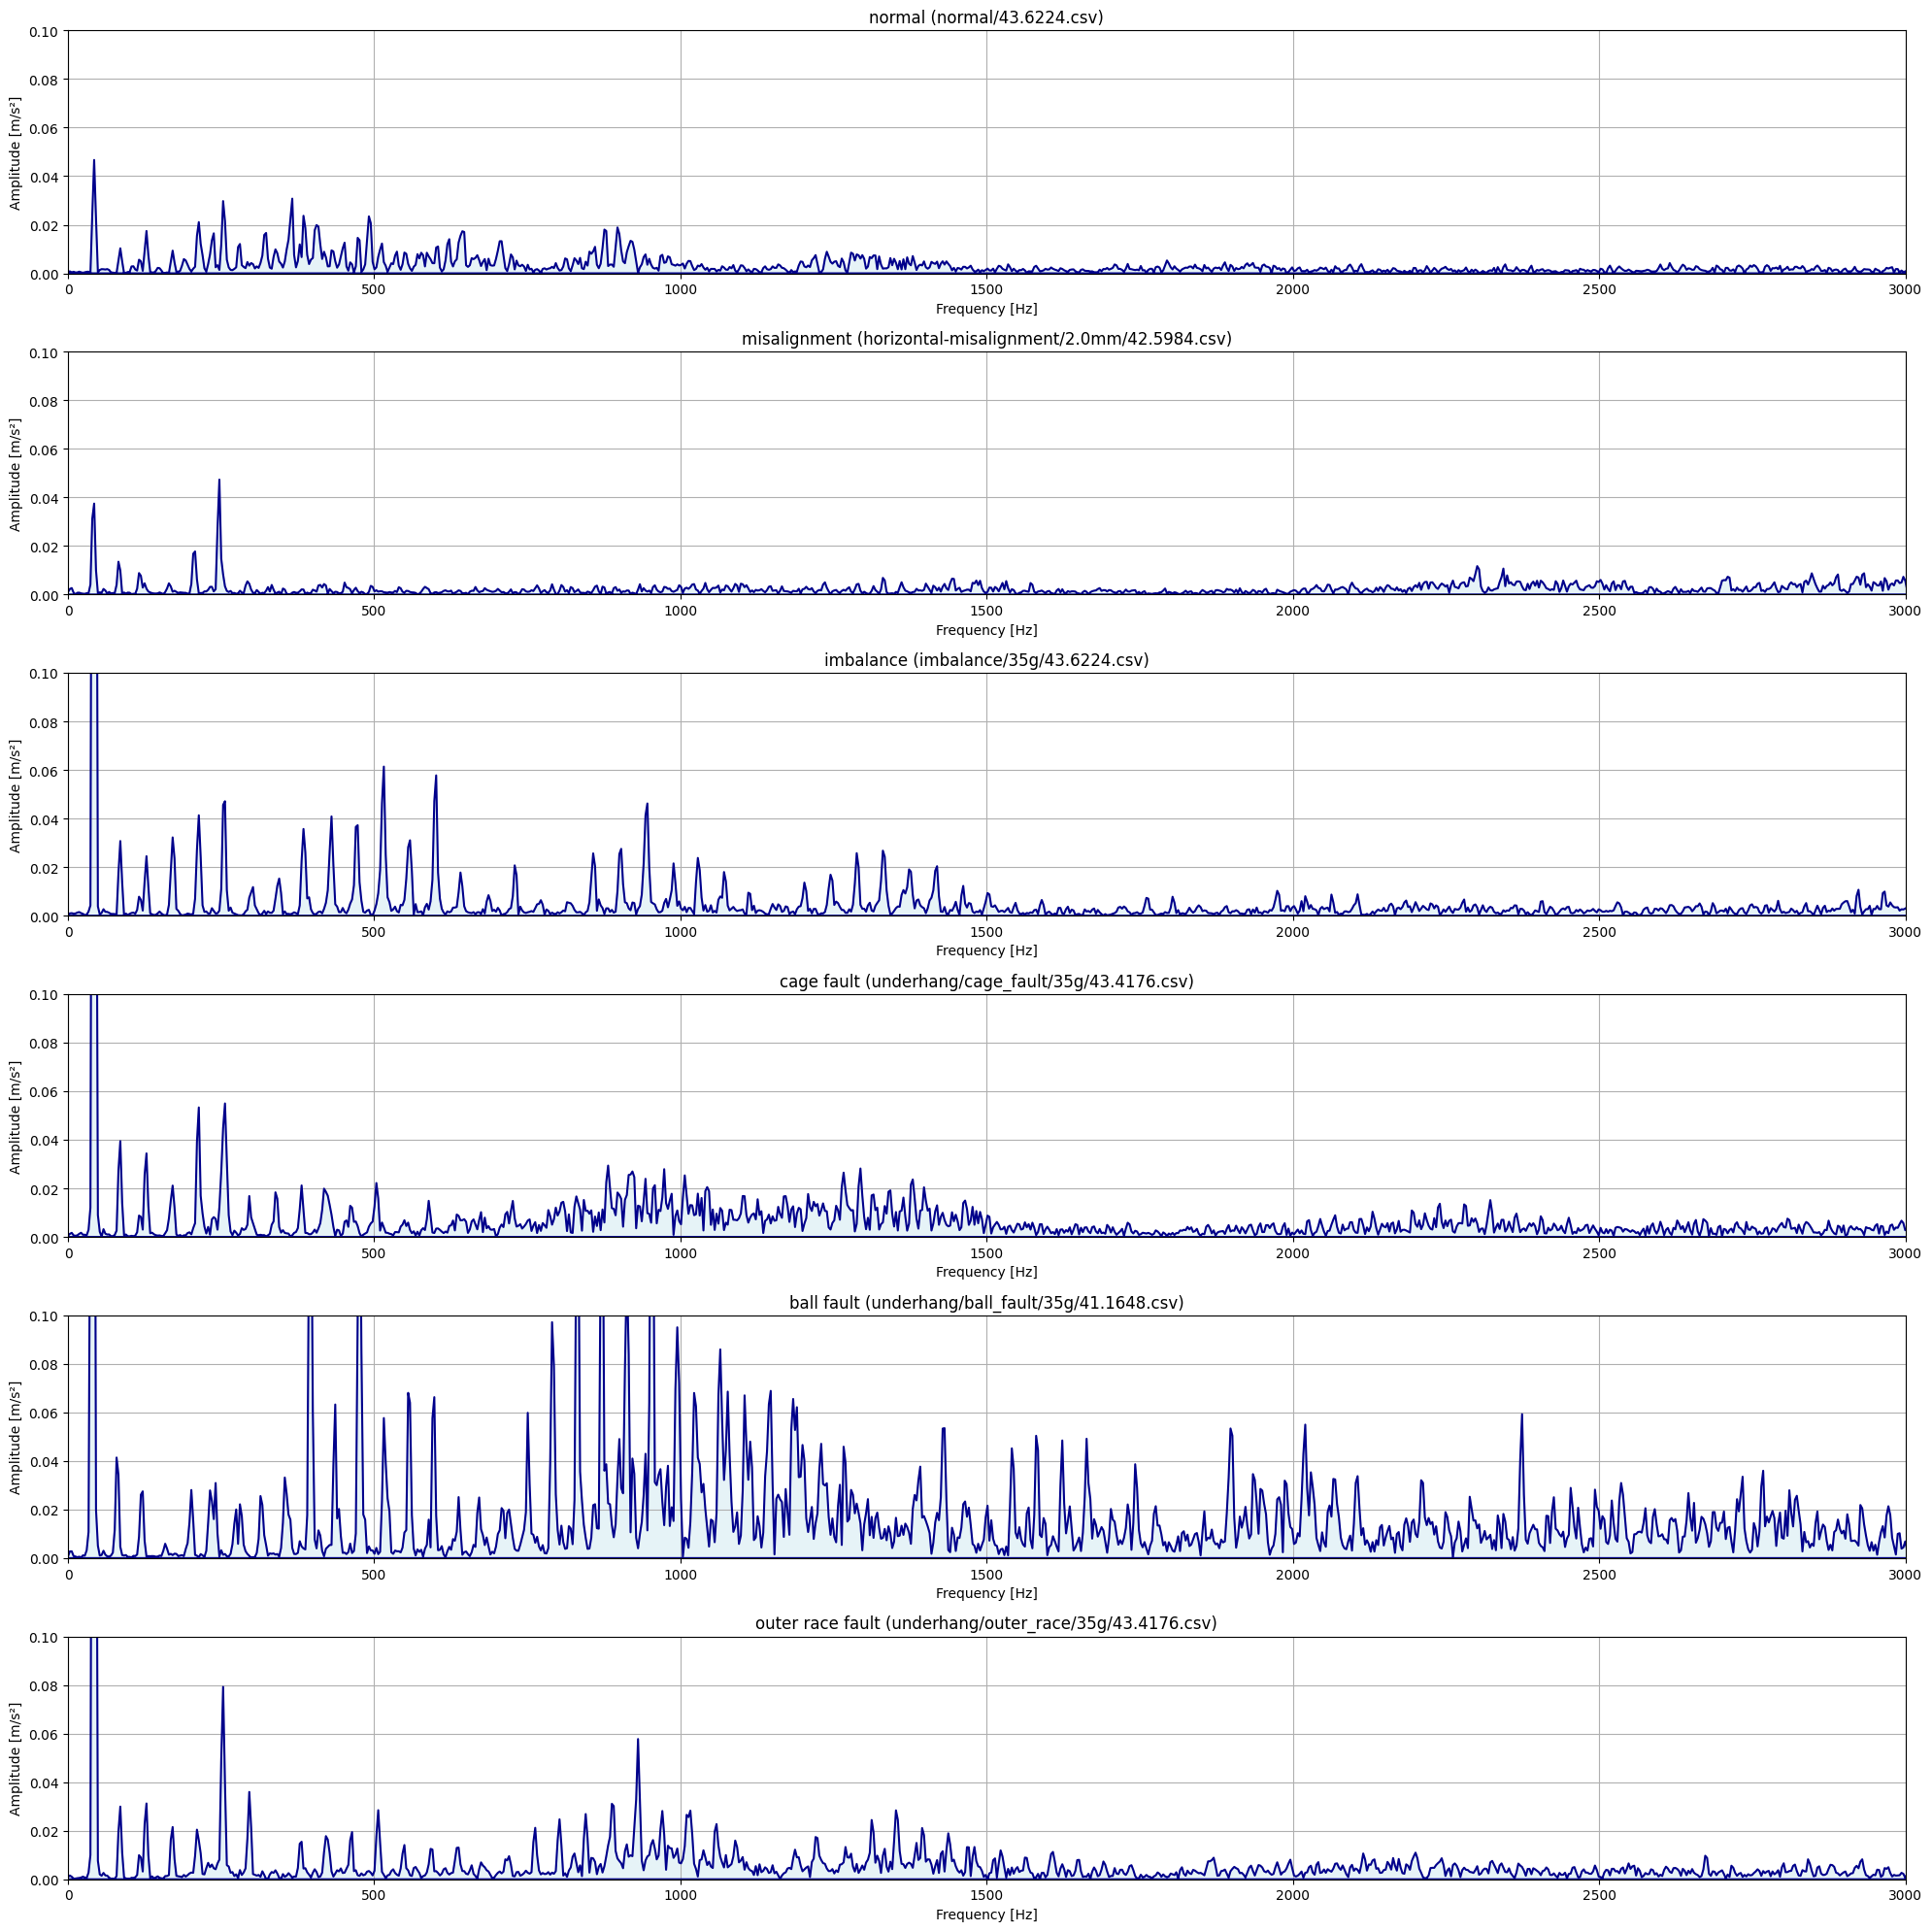
\includegraphics[width=\textwidth]{assets/design/Mafaulda-A-spectrum-Y-axis.png}
        \caption{Spectra in radial direction}
        \label{fig:design:fault-spectral-waveform}
    \end{subfigure} 
    \caption{Inner bearing vibrations (A) for each fault category with the highest fault severity at 2500 rpm}
\end{figure}

Temporal domain waveforms of the 300 ms signal slice are shown in the graphs in Figure \ref{fig:design:fault-temporal-waveform}. Subplots for radial, tangential, and axial directions are laid out in columns from left to right. Amplitudes vary with limits from $\pm 3\; \mathrm{m/s}^2$ in baseline and misalignment time series up to $\pm 11\;\mathrm{m/s}^2$ in case of severe bearing faults. 

The frequency spectrum in Figure \ref{fig:design:fault-spectral-waveform} is obtained by FFT and Hann window of length $2^{14}$. The signal chunk represents an uncertainty box with a duration of approximately 328 ms and a spectral resolution of little over 3 Hz. The graph has been cropped in both axes to make the most important peaks visible.


\subsection{Statistical tests}
The statistical tests and visual checks are conducted to assess \textbf{normality and stationary} of time series. Half a second of amplitude samples are used from every sensor channel. These 25 thousand observations are downsampled tenfold to $2500$. 

\textbf{Shapiro-Wilk's test} rejects the null hypothesis (${p < 0.05}$) that data is drawn from normal distribution under most circumstances. The signal has normal distribution when it resembles pink noise lacking a regular pattern or weak exhibition of fault symptoms. \textbf{Quantile–quantile plots} confirm non-normal distribution because of the striking samples tilt to the diagonal line.

\textbf{Augmented Dickey-Fuller test} rejects the null hypothesis of unit root 
(${p < 0.001}$). The same is confirmed with the \textbf{autocorrelation} function shape. It denotes that the stochastic process is stationary as oscillation is bounded.

\section{Feature relevance}
Attributes described in section \ref{section:feature-extraction} are independently summarized from each sensor position and direction. Then similarity score of features is ascertained in relation to a predicted variable. The subset of the strongest predictors is chosen based on the order of their perceived importance.

\subsection{Feature extraction}
Each file in the MaFaulDa contains six accelerometer channels. In the feature extraction process, the sequence of samples is split into five parts or 1-second intervals. The portions are passed through the same DC removal and low pass filters as previously. The rotational speed is derived from speedometer pulses within the chunk.

Signal chunks are converted afterward into \textbf{10 temporal and 11 spectral features}. Welch's method for spectrum density estimation averaging over $2^{14}$ long FFT segments after Hann windowing is the source for spectral features. The reference implementation of feature calculation is crafted according to mathematical formulas atop of Python packages \emph{SciPy}\footnote{SciPy: \url{https://scipy.org/}} and \emph{Time Series Feature Extraction Library} (TSFEL)\footnote{TSFEL: \url{https://tsfel.readthedocs.io/}}.

The Euclidian norm of feature in the triaxial vector eliminates reliance on the direction of measurement. Value ranges are depicted in Figure \ref{fig:design:feature-range}. 


\begin{figure}[ht]
    \centering
    \begin{subfigure}[b]{\textwidth}
        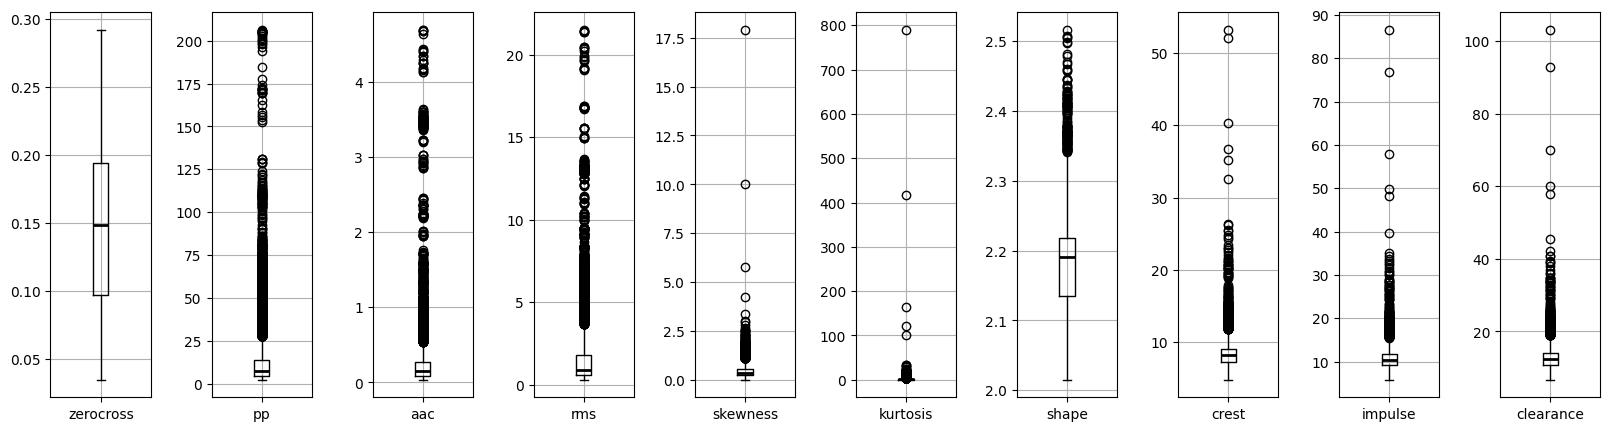
\includegraphics[width=\textwidth]{assets/design/feature-range-temporal.png}
        \caption{Temporal features}
    \end{subfigure}
    \hfill
    \begin{subfigure}[b]{\textwidth}
        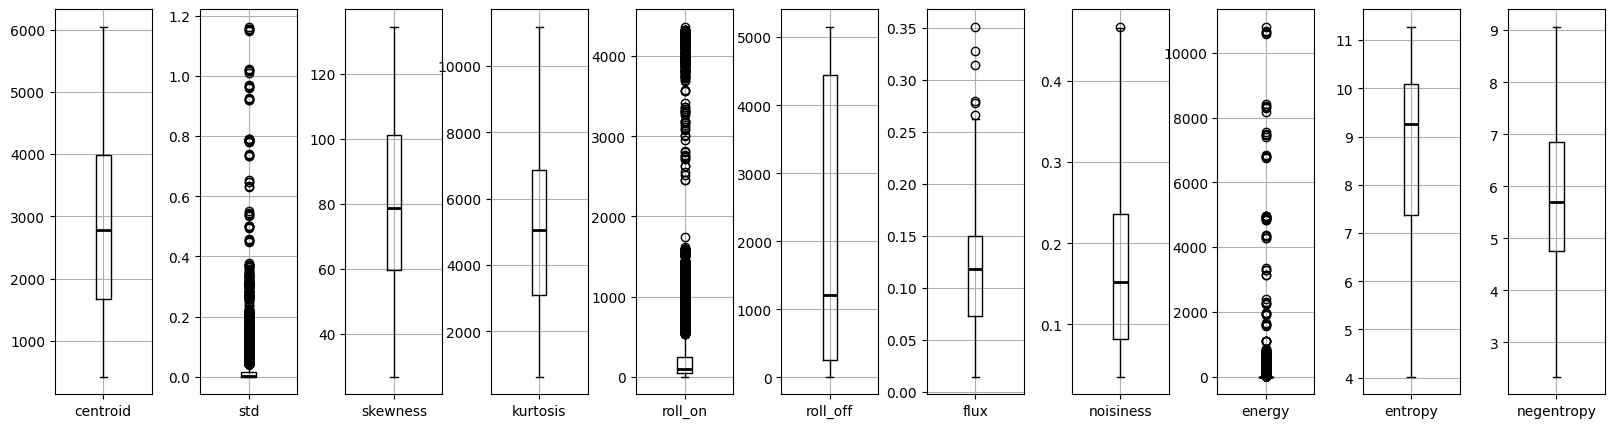
\includegraphics[width=\textwidth]{assets/design/feature-range-spectral.png}
        \caption{Spectral features}
    \end{subfigure}
    \caption{Feature value ranges in inner bearing position (A)}
    \label{fig:design:feature-range}
\end{figure}

Fault labels and their severities come from the directory structure within the dataset. The binary target variable indicating whether to initiate a warning is named to be an anomaly. Anomalies are labeled according to relative fault severity level. We decided to investigate two fault severities having levels above 0.6 and 0.9. The quantity of observation by fault and anomaly severity is shown in Table \ref{tab:observation-counts}. The dataset is substantially unbalanced.

\begin{table}[ht]
\centering
\renewcommand{\arraystretch}{1.2}
\begin{tabular}{rrrrrllll}
\cline{1-3}
\multicolumn{1}{|l|}{\textbf{Fault}}                                                                                          & \multicolumn{1}{l|}{\textbf{Inner bearing (A)}} & \multicolumn{1}{l|}{\textbf{Outer bearing (B)}} \\ \cline{1-3}
\multicolumn{1}{|r|}{\textbf{normal}}                 & \multicolumn{1}{r|}{49 (3\%)}                   & \multicolumn{1}{r|}{49 (4\%)}                    \\ \cline{1-3}
\multicolumn{1}{|r|}{\textbf{misalignment}}           & \multicolumn{1}{r|}{498 (35\%)}                 & \multicolumn{1}{r|}{498 (36\%)}                  \\ \cline{1-3}
\multicolumn{1}{|r|}{\textbf{imbalance}}              & \multicolumn{1}{r|}{333 (23\%)}                 & \multicolumn{1}{r|}{333 (24\%)}                  \\ \cline{1-3}
\multicolumn{1}{|r|}{\textbf{cage fault}}             & \multicolumn{1}{r|}{188 (13\%)}                 & \multicolumn{1}{r|}{188 (13\%)}                  \\ \cline{1-3}
\multicolumn{1}{|r|}{\textbf{ball fault}}             & \multicolumn{1}{r|}{186 (13\%)}                 & \multicolumn{1}{r|}{137 (10\%)}                  \\ \cline{1-3}
\multicolumn{1}{|r|}{\textbf{outer race fault}}       & \multicolumn{1}{r|}{184 (13\%)}                 & \multicolumn{1}{r|}{188 (13\%)}                  \\ \cline{1-3}

\multicolumn{1}{|l|}{\textbf{Anomaly (> 0.6)}}                                                                                          & \multicolumn{1}{l|}{\textbf{Inner bearing (A)}} & \multicolumn{1}{l|}{\textbf{Outer bearing (B)}} \\ \cline{1-3}
\multicolumn{1}{|r|}{\textbf{False}}                                                                            & \multicolumn{1}{r|}{837 (58\%)}                 & \multicolumn{1}{r|}{831 (60\%)}          \\ \cline{1-3}
\multicolumn{1}{|r|}{\textbf{True}}                                                                             & \multicolumn{1}{r|}{601 (42\%)}                 & \multicolumn{1}{r|}{562 (40\%)}          \\ \cline{1-3}

\multicolumn{1}{|l|}{\textbf{Anomaly (> 0.9)}}                                                                                          & \multicolumn{1}{l|}{\textbf{Inner bearing (A)}} & \multicolumn{1}{l|}{\textbf{Outer bearing (B)}} \\ \cline{1-3}
\multicolumn{1}{|r|}{\textbf{False}}                                                                            & \multicolumn{1}{r|}{1227 (85\%)}                 & \multicolumn{1}{r|}{1197 (86\%)}         \\ \cline{1-3}
\multicolumn{1}{|r|}{\textbf{True}}                                                                             & \multicolumn{1}{r|}{211 (15\%)}                 & \multicolumn{1}{r|}{196 (14\%)}         \\ \cline{1-3}
\multicolumn{1}{|r|}{\textbf{Total}}                                                                            & \multicolumn{1}{r|}{\textbf{1438} (100\%)}                       & \multicolumn{1}{r|}{\textbf{1393} (100\%)}               \\ \cline{1-3}
\end{tabular}
\caption{Label count for whole MaFaulDa dataset with recordings split to 5 chunks}
\label{tab:observation-counts}
\end{table}

Pearson's correlation of features to rpm is very low in the whole dataset. In the temporal domain, the correlation coefficient is within an interval of -0.08 to 0.26. In the spectral domain, the correlation to rpm for all FFT window sizes from $2^8$ up to $2^{14}$ is mostly very low from -0.14 up to 0.26, except for centroid being around 0.35.

The correlation among features can reduce prediction power if a pair is elected where $|\mathrm{corr}| > 0.95$. The feature is not added to the subset when the threshold is exceeded. High correlations are more substantial in the temporal domain that are present in these pairs (ordered from the most correlated): \{std, rms\}, \{pp, max\}, \{crest, margin\}, \{impulse, std\}, \{impulse, rms\}. In the spectral domain set \{skewness, kurtosis\} has a strong correlation.

It is assumed that data points spread in each dimension of the feature space could distinguish groups well. The variables that the best explain after min-max scaling total dataset variance in the temporal domain are shape (29\%), rms, std, max, and p-p (each around 15\%). In the spectral domain, variance is the best explained by roll-off (28\%), entropy, skewness, centroid, and kurtosis (each around 12\%).
\begin{figure}[h!]
    \centering
    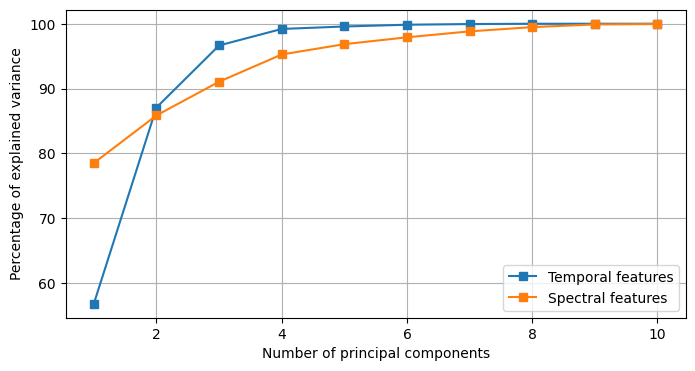
\includegraphics[width=0.8\textwidth]{assets/design/pca-explained-variance.png}
    \caption{Number of principal components to cumulative explained variance percentage in the inner bearing position}
    \label{fig:design:pca-explained-variance} 
\end{figure}

The variables are also more inter-correlated in the temporal domain shown by principal components analysis. For 95\% of the explained variance of PCA 3 components (98.69\%) are needed in the temporal domain whereas 4 in the spectral domain (95.26\%). Figure \ref{fig:design:pca-explained-variance} visualizes cumulative explained variance with an increasing number of principal components. 

\begin{figure}[h!]
    \centering
    \begin{subfigure}[b]{0.49\textwidth}
        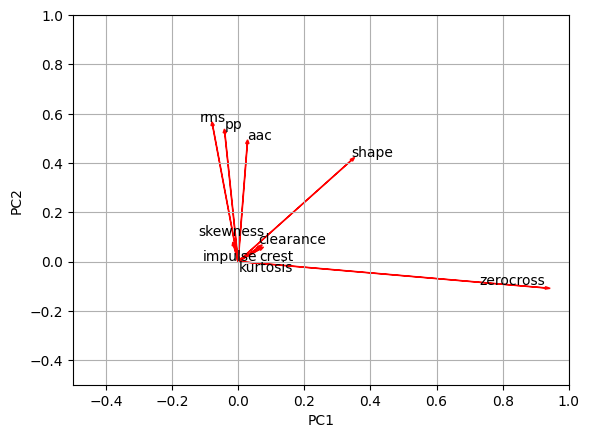
\includegraphics[width=\textwidth]{assets/design/pca-loading-plot-temporal.png}
        \caption{Temporal features}
    \end{subfigure}
    \hfill
    \begin{subfigure}[b]{0.49\textwidth}
        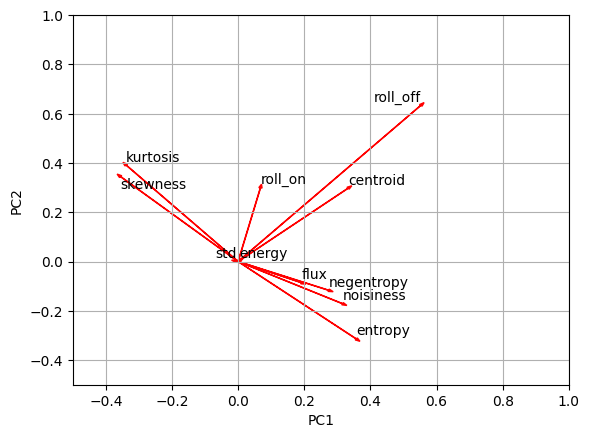
\includegraphics[width=\textwidth]{assets/design/pca-loading-plot-spectral.png}
        \caption{Spectral features}
    \end{subfigure}
    \caption{PCA loading plots for min-max scaled features from the inner bearing position}
    \label{fig:design:pca-loading-plot} 
\end{figure}

PCA efficiently expresses attributes in less dimensional space, but the resulting linear combination is hard to comprehend for explaining decisions. Loading plots of PCA (Fig. \ref{fig:design:pca-loading-plot}) illustrate correlations of features to two principal components. The first PC in the temporal domain focuses more on amplitude range: \emph{max, rms, pp, std}. The second PC mainly describes the impulsiveness of the waveform: \emph{shape, impulse, crest, margin}. 

However, the groups are not as clear cut for spectral features. Overall chaos in spectra can be attributed to PC1: \emph{flux, entropy, negentropy, noisiness}, and the shape of frequency distribution to PC2: \emph{roll-on, roll-off, centroid}.


\subsection{Data volume savings}
The apparent advantage of feature discovery is reducing the amount of data downstream. Data compression must occur on edge devices to enable the utilization of wireless low-power wide area networks (LPWAN). The protocol stack may differ, so goodput is compared without node configuration metadata and keepalive messages. 

Machinery monitoring system relies on determining several parameters:
\begin{itemize}
\itemsep0pt
\item \textbf{Number of source channels} ($S$): is comprised of the number of monitored machines, measurement locations for sensors, and active sensor axes.
\item \textbf{Sampling frequency} ($f_s$): is set based on the linear response of the accelerometer, the types of faults intended for detection, and how soon they should be noticed after they arise. The higher required sensitivity means a higher sampling rate derived according to the Nyquist theorem. At a minimum, it should be 15 kHz to 20 kHz.
\item \textbf{Interval between successive measurements} ($T$): specifies the minimal response time to sudden failure. The more critical the machine is, interval should be shorter. The bigger the machine parts, the slower the defect evolves.
\item \textbf{Duration of valid recording} ($D$): is the captured snapshot of machine unaltering behavior associated with a timestamp. Duration should cover at least 3 windows for spectral estimation. The spectral resolution of 1 Hz amounts to 3 seconds of signal under such assumptions.
\item \textbf{Number of extracted features} ($F$): are ideally key trend indicators pointing to symptoms of common malfuctions. We aim for total of 6 features.
\end{itemize}

Equation \ref{equ:compression-ratio-features} expresses the lossy compression ratio ($\mathcal{C}$) formula if trend indicators are stored instead of full recording. The number of raw channels ($S_{\mathrm{in}}$) can differ from those extracted in features ($S_{\mathrm{out}}$). Parameter $D = 0.5$ when we use frequency bins with 1 Hz resolution.

\myequations{Lossy compression ratio with features}
\begin{ceqn}\begin{align} \label{equ:compression-ratio-features}
\mathcal{C} = \frac{D \cdot f_s \cdot S_{\mathrm{in}}}{F \cdot S_{\mathrm{out}}}
\end{align}\end{ceqn}

\textbf{Compression ratio} for MaFaulDa dataset compared to all 21 extracted features in 3 dimensions is 2381:1. In case 6 features are kept, the compression is 25000:1, which is a saving of the original data amount of 99.996\%.

As an example to approximate required network goodput and storage in practice, we consider continuous vibration \textbf{monitoring for municipal water pumping station}. The station has 3 pumps and matching 3 electric induction motors. 

A pump and motor pair have 4 bearings together for drive end and non-drive end positions. Each position has a sensor mounted in 3 directions that makes a total of \emph{36 source channels}. The sampling frequency on each position is set to \emph{20 kHz}. The recordings have \emph{duration of 5 seconds} and are triggered regularly every 1 hour (\emph{8760 times per year}).

In a year the system gathers 31.54 Gs (gigasamples) which is 58.74 GiB with 16-bit ADC resolution. Reasonably precise spectral estimation with 10 thousand bins needs 3.15 Gs per year. On the other hand, 6 features out of each channel keep only 1.89 Ms per year for a lossy compression ratio of 16667:1. Low data volumes potentially enable feature selection and models to be offloaded directly to edge devices. The entire machine's history can be kept in a small flash memory module.

\subsection{Feature selection}
The objective of feature selection is to find a subset of the most relevant predictors in each domain. As a starting point, the set consists of 3 non-correlated attributes under diverse conditions. Ultimately a number of chosen features is to be tweaked to increase prediction accuracy. Four criteria are combined to put together 24 scenarios that filter rows from MaFaulDa:
\begin{itemize}
\itemsep0pt
\item \textbf{online}: boolean selector that influences whether metrics are calculated in batch or incremental fashion,
\item \textbf{placement}: chooses between bearing ``A'' and bearing ``B'',
\item \textbf{target variable}: selects column out of ``fault'', ``anomaly60'', ``anomaly90'' against which similarity is judged,
\item \textbf{rotational speed limit}: chosses whether only observations occuring within predermined range $2500 \pm 500$ rpm are filtered.
\end{itemize}

In feature evaluation for fault prediction, we use hold-out validation in batch models and progressive valuation in online models. Classes in observations for batch models are rebalanced to the majority class with a random oversampling strategy. The training and testing set split ratio is 80 to 20. Classes for incremental learning are ordered by relative severity level and shuffled within levels. 

The best group of attributes is elected based on a training set with multiple methods. We compute the mean of absolute value from point-biserial correlation, F statistic, and mutual information to the predicted variable. The features are then ordered in descending order of the received score. These individual ranks are combined by rank product to create an ensemble out of the metrics. Reference implementation of feature selection metrics uses Python packages Scikit Learn\footnote{SciKit Learn: \url{https://scikit-learn.org/}} in batch learning and RiverML\footnote{RiverML: \url{https://riverml.xyz/}} for online learning.

\begin{figure}[h!]
    \centering
    \begin{subfigure}[b]{0.49\textwidth}
        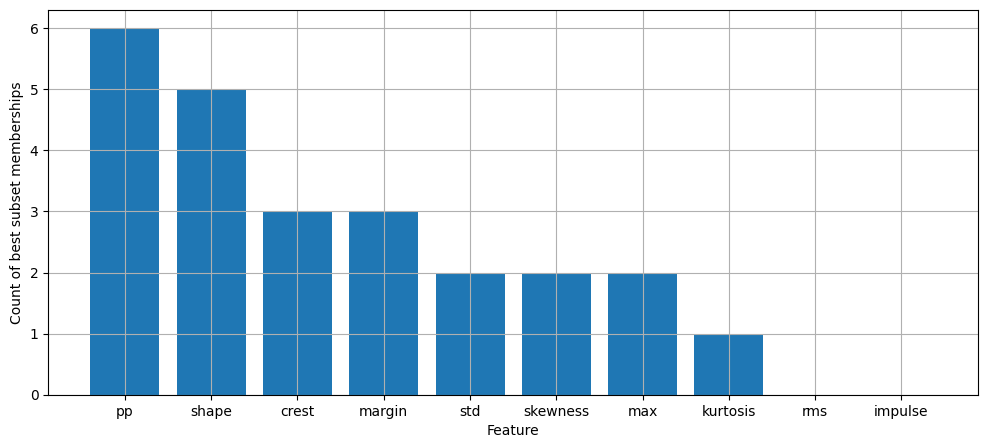
\includegraphics[width=\textwidth]{assets/design/approval-voting-temporal.png}
        \caption{Temporal domain features}
    \end{subfigure}
    \hfill
    \begin{subfigure}[b]{0.49\textwidth}
        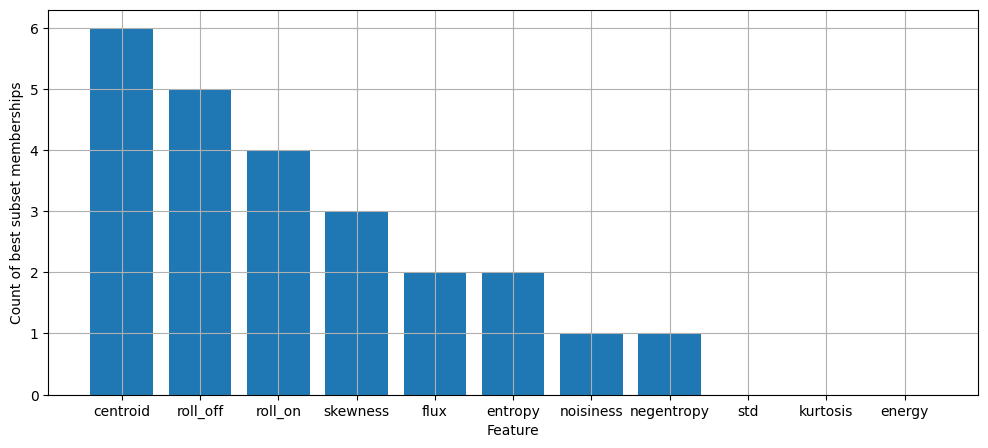
\includegraphics[width=\textwidth]{assets/design/approval-voting-spectral.png}
        \caption{Spectral domain features}
    \end{subfigure}
    \caption{Approval rating of the best triplet of features to target variable ``fault'' scored by rank product of correlation, F statistic, and mutual information.}
    \label{fig:design:approval-rating-features}
\end{figure}

The choice of features is very sensitive to experimental conditions. Tendencies are demonstrated by counting how many triplets the indicator appears in across all possible situations. The results of approval voting are shown in Figure~\ref{fig:design:approval-rating-features}. The most occurring attributes in the temporal domain are peak-to-peak, shape, and crest, and in the spectral domain, those are centroid, roll-off, and roll-on.


\section{K-nearest neighbor classifier}
We utilize the k-nearest neighbor algorithm to check machinery diagnostics abilities with reduced feature sets. kNN classifier being a lazy learner means it can be adapted easily from offline to online context. Training labels are min-max scaled and establish nearest-neighbor decision boundaries for attribute values. Voronoi diagrams can display these regions and explain the model in that way. Batch learning in kNN serves here as a target performance whose attainment is desirable with online learning.

\subsection{Batch models}
Three types of kNN model experiments run with hold-out validation in batch setting. 
First, the model learns all extracted features, so no feature selection occurs. Then, the brute-force method searches for a combination of three features with the highest training accuracy. In the end, the model performance for three attributes chosen by feature selection techniques is compared to principal components.

\begin{figure}[ht]
    \centering
    \begin{subfigure}[b]{0.49\textwidth}
        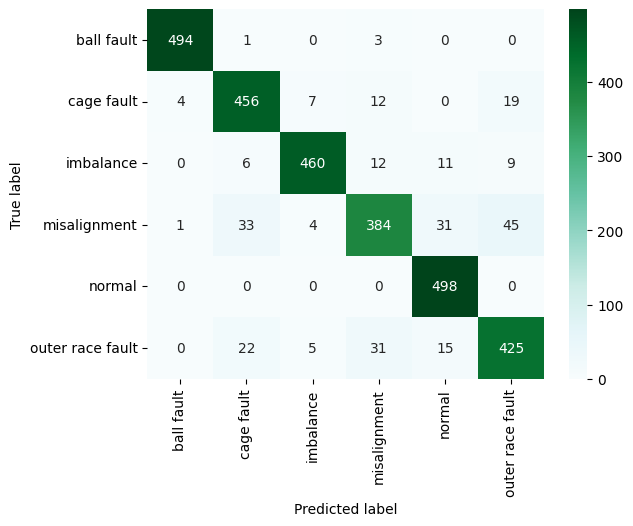
\includegraphics[width=\textwidth]{assets/design/kNN-temporal-confusion-matrix-fault.png}
        \caption{Prediction for 6 fault classes in testing set with temporal domain features}
    \end{subfigure}
    \hfill
    \begin{subfigure}[b]{0.49\textwidth}
        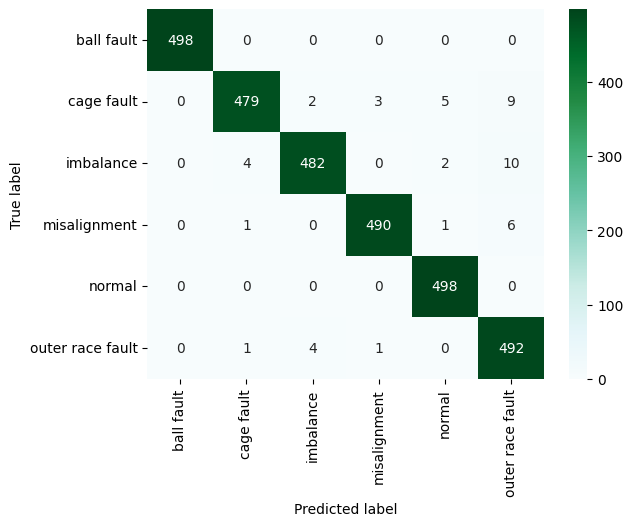
\includegraphics[width=\textwidth]{assets/design/kNN-spectral-confusion-matrix-fault.png}
        \caption{Prediction for 6 fault classes in testing set with spectral domain features}
    \end{subfigure}
    \begin{subfigure}[b]{0.49\textwidth}
        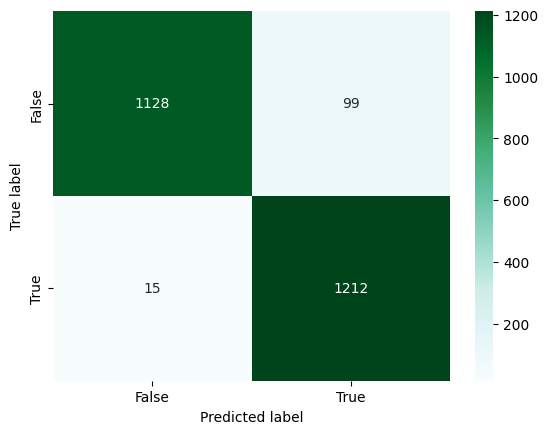
\includegraphics[width=\textwidth]{assets/design/kNN-temporal-confusion-matrix-anomaly90.png}
        \caption{Prediction of high severity anomalies in testing set with temporal domain features}
    \end{subfigure}
    \hfill
    \begin{subfigure}[b]{0.49\textwidth}
        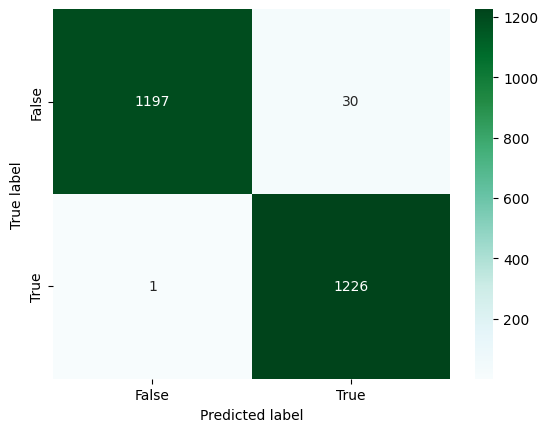
\includegraphics[width=\textwidth]{assets/design/kNN-spectral-confusion-matrix-anomaly90.png}
        \caption{Prediction of high severity anomalies in testing set with spectral domain features}
    \end{subfigure}
    \caption{Confusion matrix of kNN predictions on bearing position A}
    \label{fig:design:knn-confusion-matrix}
\end{figure}

Two models are created for the target variable in classification with all 10 temporal and 11 spectral features. The subset of records includes all rotational speeds on bearing position A. Either six fault labels or anomaly above 0.9 severity level are guessed by the model with the same hold-out validation split as before. 

Confusion matrices for fault predicion and high severity anomaly are shown in Figure \ref{fig:design:knn-confusion-matrix}. In this example, the number of k neighbors is 5, the distance metric is the Euclidian norm, and the algorithm for proximity queries is a k-d tree. The most inaccuracies in the temporal domain are between misalignment and bearing race faults. In the spectral domain, the model confuses imbalance and bearing faults. It is to be expected since mass to unbalance the shaft is hanged to simulate bearing defects. 

In anomaly prediction, the error of the first degree is 7 times more prevalent than the error of the second degree. False positives are preferable since we do not want the machine to fail prematurely and not know about it. In all cases, spectral features maintain better prediction metrics than all temporal features because of less interdependency among features. Bearing B exhibits overall worse classification performance because of more noise in the original signal.

\begin{table}[h]
\centering
\renewcommand{\arraystretch}{1.2}
\begin{adjustbox}{width=\textwidth}
\begin{tabular}{|l|l|l|rrr|rrr|}
\hline
\multirow{2}{*}{\textbf{\begin{tabular}[c]{@{}l@{}}Bearing\\ position\end{tabular}}} & \multirow{2}{*}{\textbf{\begin{tabular}[c]{@{}l@{}}Target\\ variable\end{tabular}}} & \multirow{2}{*}{\textbf{Observations}}                                             & \multicolumn{3}{l|}{\textbf{Temporal domain}}                                                                                                                                                                                                                                    & \multicolumn{3}{l|}{\textbf{Spectral domain}}                                                                                                                                                                                                                                    \\ \cline{4-9} 
                                                                                     &                                                                                     &                                                                                   & \multicolumn{1}{l|}{\textbf{\begin{tabular}[c]{@{}l@{}}Training\\ accuracy\end{tabular}}} & \multicolumn{1}{l|}{\textbf{\begin{tabular}[c]{@{}l@{}}Testing\\ accuracy\end{tabular}}} & \multicolumn{1}{l|}{\textbf{\begin{tabular}[c]{@{}l@{}}Training\\ F1 score\end{tabular}}} & \multicolumn{1}{l|}{\textbf{\begin{tabular}[c]{@{}l@{}}Training\\ accuracy\end{tabular}}} & \multicolumn{1}{l|}{\textbf{\begin{tabular}[c]{@{}l@{}}Testing\\ accuracy\end{tabular}}} & \multicolumn{1}{l|}{\textbf{\begin{tabular}[c]{@{}l@{}}Training\\ F1 score\end{tabular}}} \\ \hline
\multirow{2}{*}{A}                                                                   & Fault                                                                               & \begin{tabular}[c]{@{}l@{}}$\sum 2998$\\ 498 per class\end{tabular}  & \multicolumn{1}{r|}{0.9413}                                                               & \multicolumn{1}{r|}{0.9093}                                                              & 0.91                                                                                      & \multicolumn{1}{r|}{0.9917}                                                               & \multicolumn{1}{r|}{0.9836}                                                              & 0.98                                                                                      \\ \cline{2-9} 
                                                                                     & \begin{tabular}[c]{@{}l@{}}Anomaly\\ (0.9)\end{tabular}                               & \begin{tabular}[c]{@{}l@{}}$\sum 2454$\\ 1227 per class\end{tabular} & \multicolumn{1}{r|}{0.9668}                                                               & \multicolumn{1}{r|}{0.9535}                                                              & 0.96                                                                                      & \multicolumn{1}{r|}{0.9921}                                                               & \multicolumn{1}{r|}{0.9874}                                                              & 0.99                                                                                      \\ \hline
\multirow{2}{*}{B}                                                                   & Fault                                                                               & \begin{tabular}[c]{@{}l@{}}$\sum 2998$\\ 498 per class\end{tabular}  & \multicolumn{1}{r|}{0.8634}                                                               & \multicolumn{1}{r|}{0.7935}                                                              & 0.79                                                                                      & \multicolumn{1}{r|}{0.9207}                                                               & \multicolumn{1}{r|}{0.8765}                                                              & 0.87                                                                                      \\ \cline{2-9} 
                                                                                     & \begin{tabular}[c]{@{}l@{}}Anomaly \\ (0.9)\end{tabular}                              & \begin{tabular}[c]{@{}l@{}}$\sum 2394$\\ 1197 pre class\end{tabular} & \multicolumn{1}{r|}{0.9148}                                                               & \multicolumn{1}{r|}{0.8668}                                                              & 0.87                                                                                      & \multicolumn{1}{r|}{0.9428}                                                               & \multicolumn{1}{r|}{0.9156}                                                              & 0.92                                                                                      \\ \hline
\end{tabular}
\end{adjustbox}
\caption{kNN model performance trained on all extracted features}
\label{tab:design:all-extracted-features}
\end{table}

Accuracies and F1 scores in both bearing positions with all extracted features are shown in Table \ref{tab:design:all-extracted-features}. Models are overtrained, especially for temporal features, because of the substantial difference between accuracy on training and validation sets. Binary classification of anomaly is unsurprisingly more precise in general than multiclass case. Defect-type detection with all features reaches accuracy on the testing set above 98\% for bearing A, and above 87\% for bearing B.

Next, we exhaustively list all combinations of three features and look at the range of model performances generated. There are $\binom{n}{3}$ combinations of attribute triplets that entail 120 separate kNN models for temporal domain features and 165 for the spectral domain. The feature set with the best evaluation scores serves as a benchmark for attributes picked by selection techniques. Accuracies of kNN algorithm for different target variables are in Figure \ref{fig:design:feature-combinations-knn}. 

\begin{figure}[ht]
    \centering
    \begin{subfigure}[b]{\textwidth}
        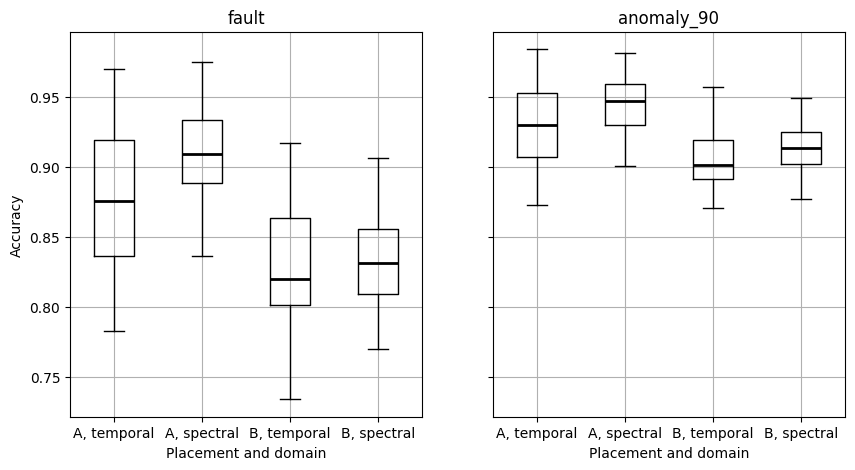
\includegraphics[width=\textwidth]{assets/design/kNN-3-features-combinations-train.png}
        \caption{Testing set}
    \end{subfigure}
    \hfill
    \begin{subfigure}[b]{\textwidth}
        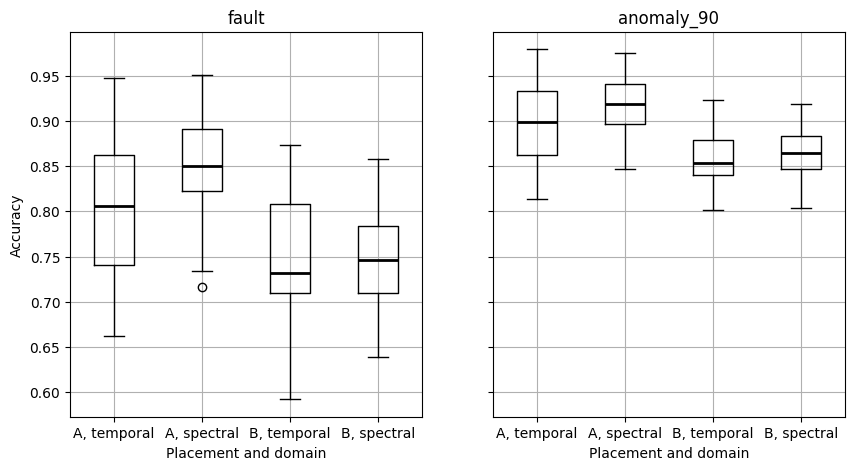
\includegraphics[width=\textwidth]{assets/design/kNN-3-features-combinations-test.png}
        \caption{Training set}
    \end{subfigure}
    \caption{Range of prediction accuracy in all kNN models with subset of 3 features. Subplots show three different predicted variables.}
    \label{fig:design:feature-combinations-knn}
\end{figure}

Features picked combinatorically for predictions are listed in Table \ref{tab:design:feature-combinations-knn}. Worst accuracies occur for temporal features in multiclass classification 86\% and 77\% depending on bearing position, as compared to 98\% and 91\% accuracy for spectral features. An improvement would come with increasing the number of features, using a different base feature set with greater discriminatory power, or using a more sophisticated model.

\begin{table}[ht!]
\centering
\renewcommand{\arraystretch}{1.2}
\begin{adjustbox}{width=\textwidth}
\begin{tabular}{|r|r|r|l|r|r|}
\hline
\multicolumn{1}{|l|}{\textbf{Place}} & \multicolumn{1}{l|}{\textbf{\begin{tabular}[c]{@{}l@{}}Target \\ variable\end{tabular}}} & \multicolumn{1}{l|}{\textbf{Domain}} & \multicolumn{1}{l|}{\textbf{Best feature triplet}} & \textbf{\begin{tabular}[c]{@{}l@{}}Training \\ accuracy\end{tabular}} & \textbf{\begin{tabular}[c]{@{}l@{}}Testing \\ accuracy\end{tabular}} \\ \hline
\multirow{4}{*}{A} & \multirow{2}{*}{\begin{tabular}[c]{@{}r@{}}anomaly\\ (0.9)\end{tabular}}              & temporal        & \{std, skewness, shape\}         & 0.9559                & 0.9328               \\ \cline{3-6} 
                   &                                               & spectral        & \{centroid, noisiness, entropy\} & 0.9818                & 0.9707               \\ \cline{2-6} 
                   & \multirow{2}{*}{fault}                        & temporal        & \{std, skewness, shape\}         & 0.9106                & 0.8591 \\ \cline{3-6} 
                   &                                               & spectral        & \{centroid, kurtosis, entropy\}  & 0.9750                & 0.9505               \\ \hline
\multirow{4}{*}{B} & \multirow{2}{*}{\begin{tabular}[c]{@{}r@{}}anomaly\\ (0.9)\end{tabular}}               & temporal        & \{std, kurtosis, pp\}            & 0.9085                & 0.8551               \\ \cline{3-6} 
                   &                                               & spectral        & \{centroid, std, roll-on\}      & 0.9495                & 0.9185               \\ \cline{2-6} 
                   & \multirow{2}{*}{fault}                        & temporal        & \{std, skewness, kurtosis\}      & 0.8369                & 0.7654 \\ \cline{3-6} 
                   &                                               & spectral        & \{centroid, std, roll-off\}     & 0.9067                & 0.8584               \\ \hline
\end{tabular}
\end{adjustbox}
\caption{Features with the highest accuracies on the training set found combinatorically}
\label{tab:design:feature-combinations-knn}
\end{table}

The features picked using the rank product method are shown in Table \ref{tab:design:best-3-features-knn}. Their prediction accuracies in kNN models are subpar to optimal sets. However, the advantage is that the feature election process is not so computationally taxing. On bearing A, validation set accuracies for fault diagnostics are 85\% and 92\%, for each of the domains. Because of the low k hyperparameter value, models are overtrained either way.

\begin{table}[ht!]
\centering
\renewcommand{\arraystretch}{1.2}
\begin{adjustbox}{width=\textwidth}
\begin{tabular}{|r|r|r|l|r|r|}
\hline
\multicolumn{1}{|l|}{\textbf{Place}} & \multicolumn{1}{l|}{\textbf{\begin{tabular}[c]{@{}l@{}}Target \\ variable\end{tabular}}} & \multicolumn{1}{l|}{\textbf{Domain}} & \multicolumn{1}{l|}{\textbf{Best feature triplet}} & \textbf{\begin{tabular}[c]{@{}l@{}}Train \\ accuracy\end{tabular}} & \textbf{\begin{tabular}[c]{@{}l@{}}Test \\ accuracy\end{tabular}} \\ \hline
\multirow{4}{*}{A} & \multirow{2}{*}{\begin{tabular}[c]{@{}r@{}}anomaly\\ (0.9)\end{tabular}}                & temporal        & \{shape, std, rms\}               & 0.9333                                       & 0.8916                                      \\ \cline{3-6} 
                   &                                               & spectral        & \{centroid, flux, entropy\}       & 0.9654                                       & 0.9474                                      \\ \cline{2-6} 
                   & \multirow{2}{*}{fault}                        & temporal        & \{std, shape, max\}               & 0.9048                                       & 0.8544                                      \\ \cline{3-6} 
                   &                                               & spectral        & \{roll-off, centroid, skewness\} & 0.9504                                       & 0.9210                                      \\ \hline
\multirow{4}{*}{B} & \multirow{2}{*}{\begin{tabular}[c]{@{}r@{}}anomaly\\ (0.9)\end{tabular}}              & temporal        & \{std, shape, crest\}             & 0.8961                                       & 0.8505                                      \\ \cline{3-6} 
                   &                                               & spectral        & \{std, noisiness, entropy\}       & 0.9265                                       & 0.8843                                      \\ \cline{2-6} 
                   & \multirow{2}{*}{fault}                        & temporal        & \{pp, crest, skewness\}           & 0.8194                                       & 0.7380                                      \\ \cline{3-6} 
                   &                                               & spectral        & \{centroid, roll-on, roll-off\} & 0.8914                                       & 0.8390                                      \\ \hline
\end{tabular}
\end{adjustbox}
\caption{Three chosen features with rank product of correlation, F statistic, mutual information and their associated kNN accuracies.}
\label{tab:design:best-3-features-knn}
\end{table}

Lowering the number of attributes allows visualization of labels in planar scatter plots. The data points in 3-dimensional cross sections are colored by true fault classes of all severities in Figure \ref{fig:design:feature-space-scatter}. We observe the inability to separate faults by linear boundaries in given feature spaces and the noncompactness of clusters. 

Cluster overlaps of various defect types are also confirmed by silhouette scores around zero. Therefore, the k hyperparameter cannot be increased much, as it would cause the merge of mutually confused categories. Low-severity faults should be relabeled as a class without fault to watch out just for alert conditions.

\begin{figure}[ht]
    \centering
    \begin{subfigure}[b]{\textwidth}
        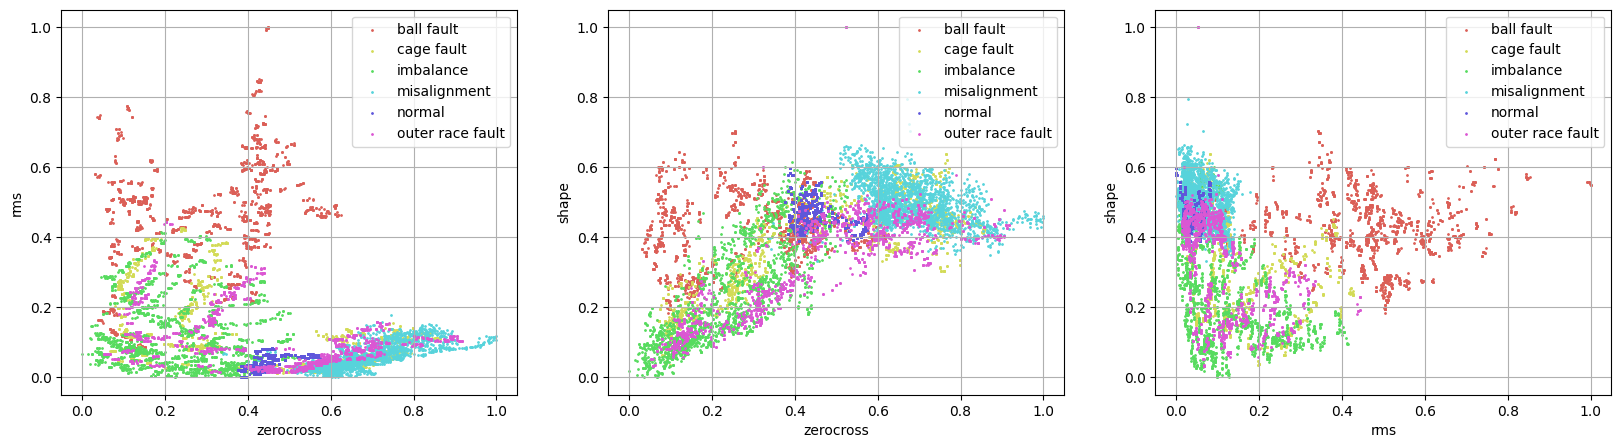
\includegraphics[width=\textwidth]{assets/design/best-features-scatter-fault-A-temporal.png}
        \caption{Temporal domain features}
    \end{subfigure}
    \hfill
    \begin{subfigure}[b]{\textwidth}
        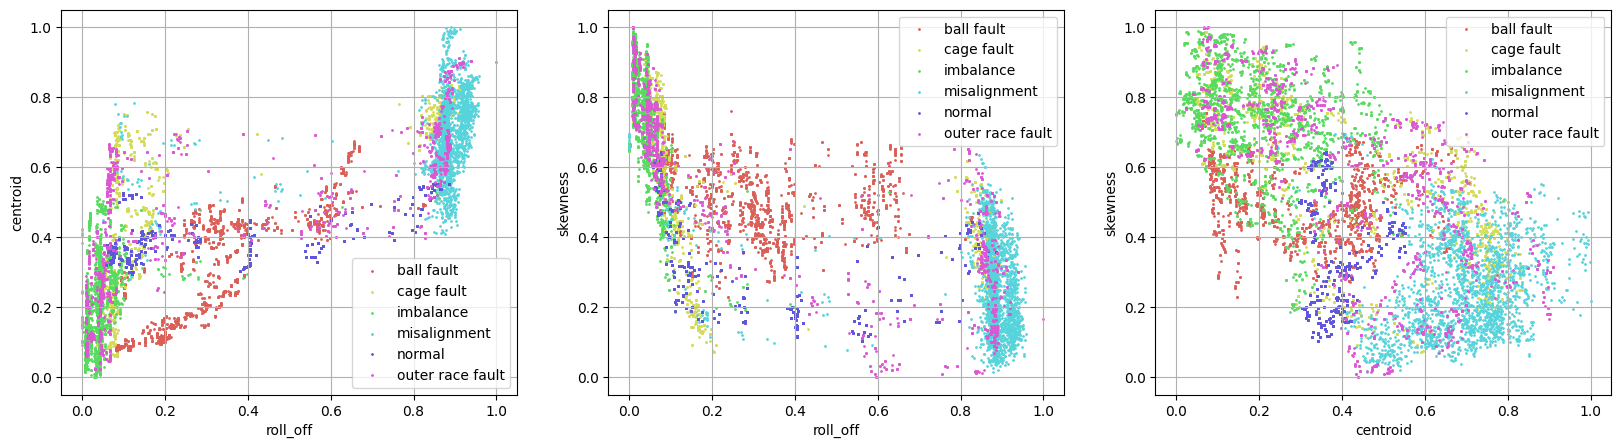
\includegraphics[width=\textwidth]{assets/design/best-features-scatter-fault-A-spectral.png}
        \caption{Spectral domain features}
    \end{subfigure} 
    \caption{Cross sections of 3-dimensional feature spaces with ground truth labels for best attributes. Features are chosen by rank product method.}
    \label{fig:design:feature-space-scatter}
\end{figure}

Model performance of kNN algorithm preceeded by variety of feature selection methods is compared in Figure \ref{fig:design:knn-accuracy-batch}. Best combination of three features achieves always better than when the model is trained on all features. This has to do with curse of dimensionality phenomenon. 

\begin{figure}[ht]
    \centering
    \begin{subfigure}[b]{\textwidth}
        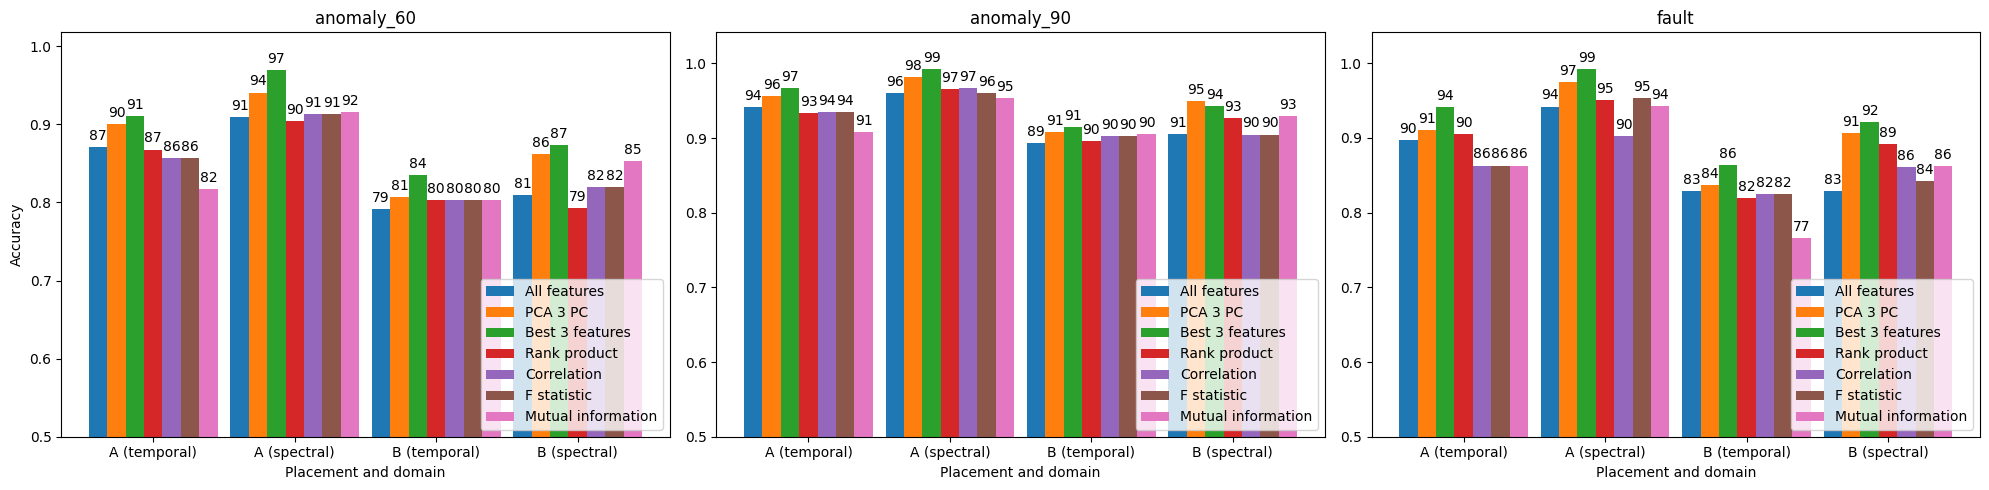
\includegraphics[width=\textwidth]{assets/design/kNN-feature-selection-predictions-train.png}
        \caption{Testing set}
    \end{subfigure}
    \hfill
    \begin{subfigure}[b]{\textwidth}
        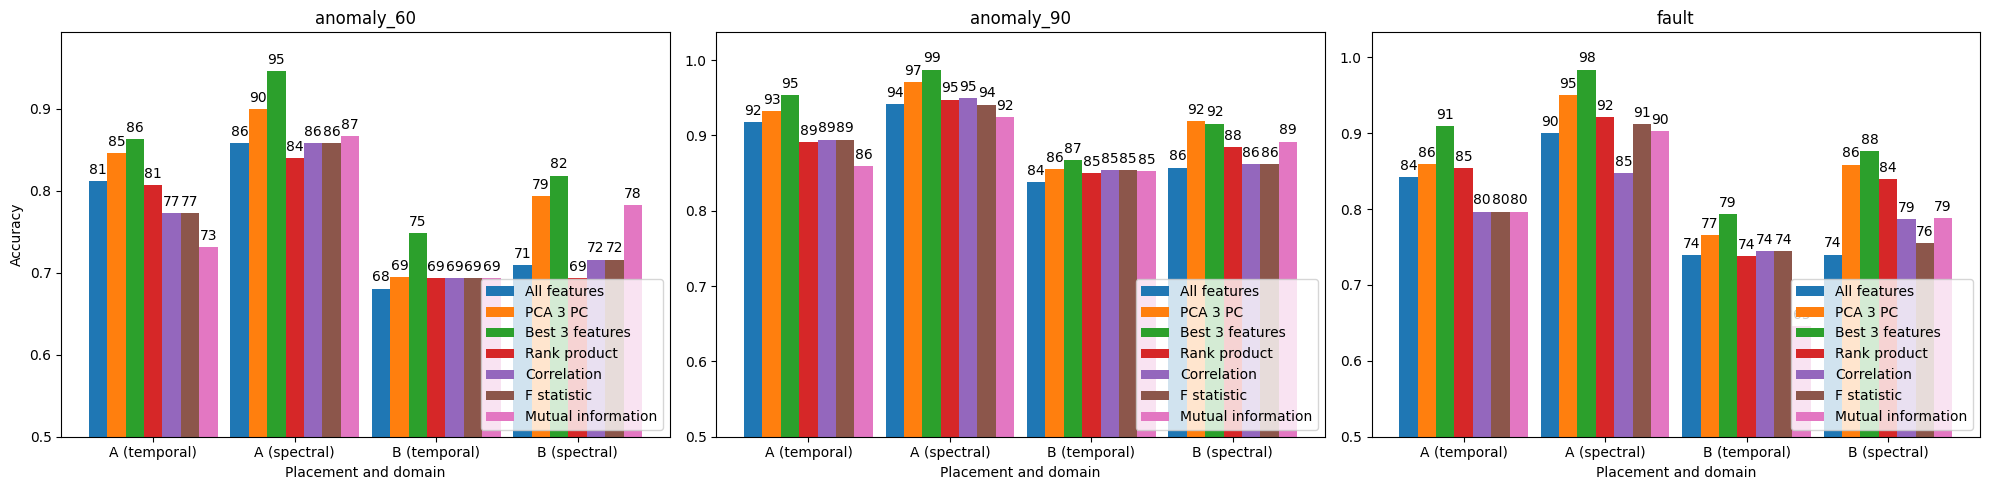
\includegraphics[width=\textwidth]{assets/design/kNN-feature-selection-predictions-test.png}
        \caption{Training set}
    \end{subfigure} 
    \caption{Batch kNN algorithm prediction accuracy with various feature sets.}
    \label{fig:design:knn-accuracy-batch}
\end{figure} 

We suspected that the PCA property of maximizing variances in each of the few dimensions would support more separation of clustered groups and would be beneficial in classification. The bar chart supports this assumption. PCA always produces greater model accuracies than any other method of feature selection. The rank product of the three scoring techniques is not better every time, but it balances out aggregated methods to achieve more stable results across testing sets. 

In every instance, a subset of spectral features is responsible for better accuracy than a subset of temporal features. Presumably, it is so because of many correlated pairs of attributes in the temporal domain. Further tests should be made to determine optimal feature subsets and the impact of altering the feature election process.


\subsection{Online models}
Online learning imitates hardened conditions for machinery diagnostics that appear in deployment. Delayed provision or omission of actual labels undoubtedly degrades the reliability of the classification. The question is how quickly the accuracy approaches the optimal one from the nearest neighbors trained in batch and what the effect of routine difficulties in the ongoing labeling process is.

The kNN models in incremental learning experiments learn on the same base training dataset for bearing position A and with all extracted features as in batch context. In this manner, we can compare the training accuracies in the last sample for both models. kNN is set to 5 nearest neighbors and proximity metric of Euclidian distance. Online learning metrics are evaluated in progressive valuation on a dataset that is left unbalanced.

The \textbf{stream of events is sorted} by rising severity levels (Fig.~\ref{fig:design:online-count-severity-level}) which ensures steady increments in label counts throughout the whole duration of the simulation (Fig.~\ref{fig:design:online-event-order}). This constructed event sequence is a bit unrealistic because all types of faults never begin to appear simultaneously with equal strengths. It is meant to approximate the gradual overall degradation of the machine. 

\begin{figure}[ht]
    \centering
    \begin{subfigure}[b]{0.49\textwidth}
        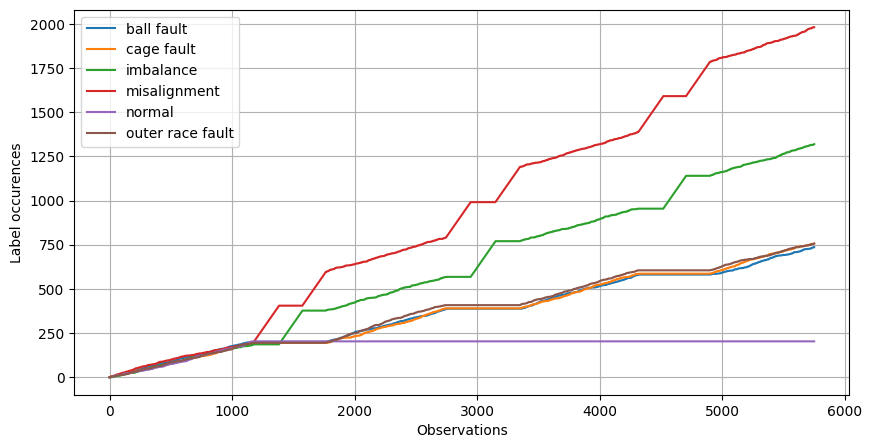
\includegraphics[width=\textwidth]{assets/design/Online-event-ordering-fault-train.png}
        \caption{Event ordering of faults}
        \label{fig:design:online-event-order}
    \end{subfigure}
    \hfill
    \begin{subfigure}[b]{0.49\textwidth}
        \includegraphics[width=\textwidth]{assets/design/Online-severity-levels.png}
        \caption{Fault severity levels ordering}
        \label{fig:design:online-count-severity-level}
    \end{subfigure}
    \caption{Label sequencing for progressive evaluation}
\end{figure}

Major breaking points in the stream are after 1171 observations out of 5751, where all 203 normal conditions are consumed in the training process. Counters of other faults show that model prediction are skewed towards more represented classes of imbalance and misalignement. The uneven evolution of category counts in a stream impacts the development of accuracy in the remaining experiments. The training accuracies of comparable batch models are 94.13\% \emph{(temporal features)} and 99.17\% \emph{(spectral features)}.
	
During gradual learning, the correct label is supplied after a fixed period passes after its prediction. This \textbf{sliding window} simulation examines accuracy every 100 iterations. Wait times before revealing the actual class associated with the sample are 1, 50, 100, or 250 steps (Fig.~\ref{ffig:design:online-fault-delay-sliding}). 


\begin{figure}[ht]
    \centering
    \begin{subfigure}[b]{\textwidth}
        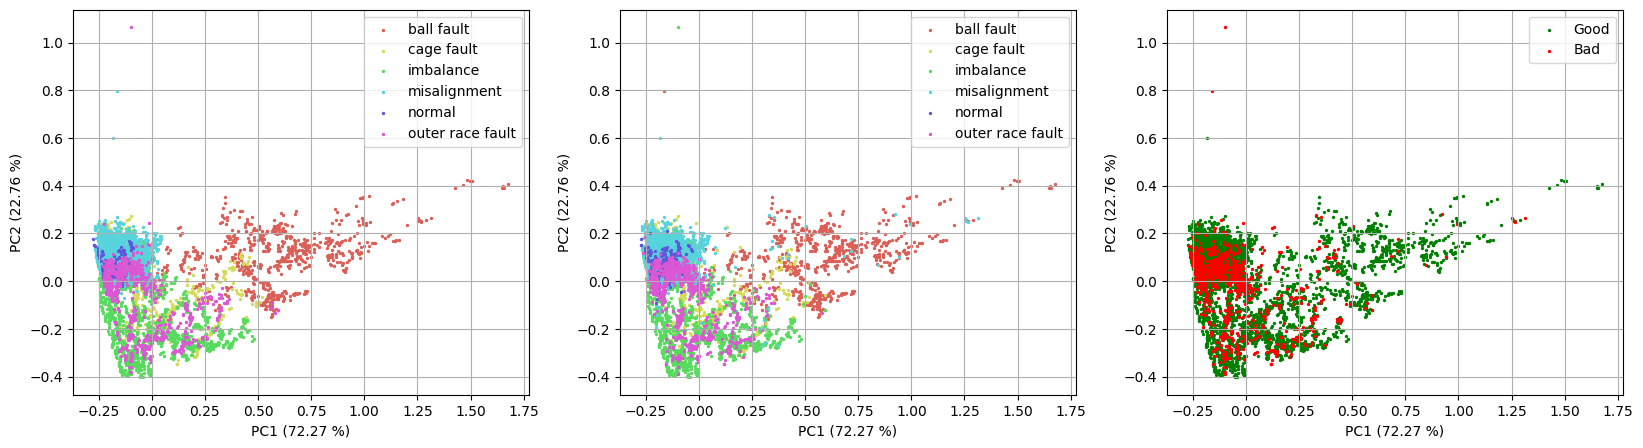
\includegraphics[width=\textwidth]{assets/design/pca-scatter-online-fault-temporal.png}
        \caption{Principal components from temporal domain features}
    \end{subfigure}
    \hfill
    \begin{subfigure}[b]{\textwidth}
        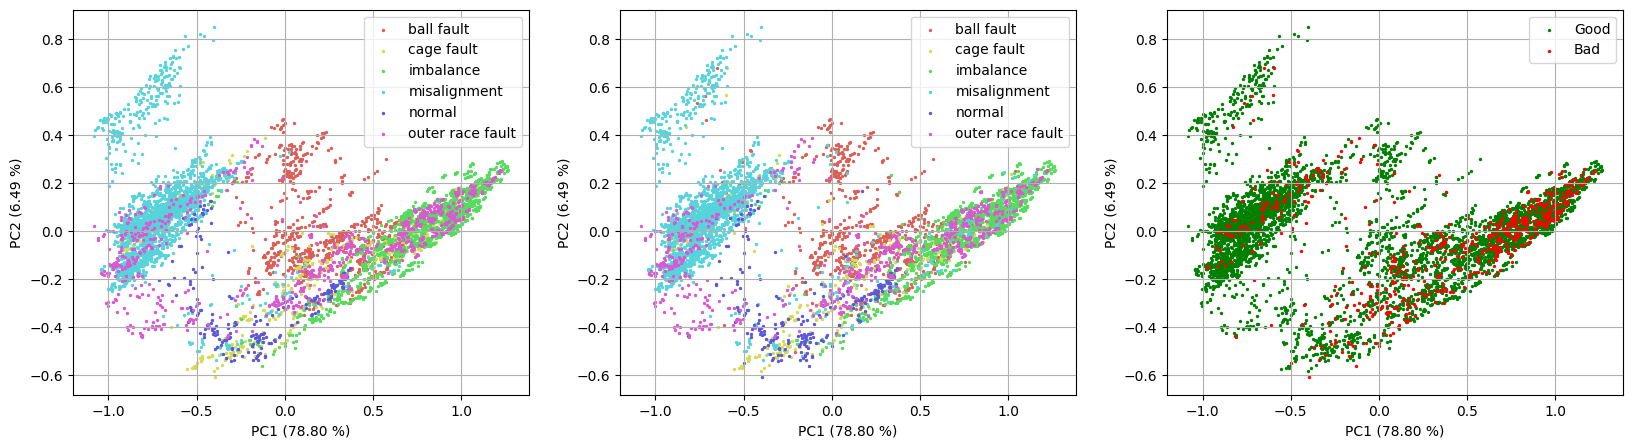
\includegraphics[width=\textwidth]{assets/design/pca-scatter-online-fault-spectral.png}
        \caption{Principal components from spectral domain features}
    \end{subfigure}
    \caption{Classification labels in incremental learning \emph{(from left)}: true labels, predicted labels, mistakes in predictions.}
    \label{fig:design:scatter-plot-online}
\end{figure}

Accuracies after sequentially seeing all samples are 82.92\% \emph{(temporal)} and 89.11\% \emph{(spectral)} when labels are shown instantly. Scatter plots in Figure~\ref{fig:design:scatter-plot-online} visualize mistakes in predictions projected onto two principal components. Labeling delay of 250 observations causes accuracies to drop to 70.51\% \emph{(temporal)} and 78.81\% \emph{(spectral)}. Accuracy better than 50\% is achieved 200 steps sooner in the spectral domain than in the temporal domain.
	
\begin{figure}[ht]
    \centering
    \begin{subfigure}[b]{0.49\textwidth}
        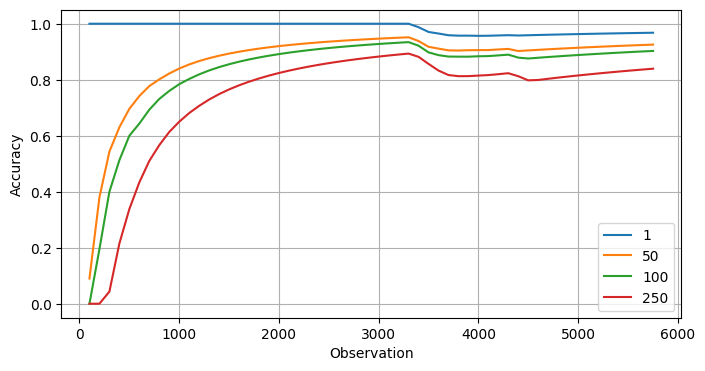
\includegraphics[width=\textwidth]{assets/design/gradual-learning-accuracy-delay-temporal-domain-fault.png}
        \caption{Temporal domain features}
    \end{subfigure}
    \hfill
    \begin{subfigure}[b]{0.49\textwidth}
        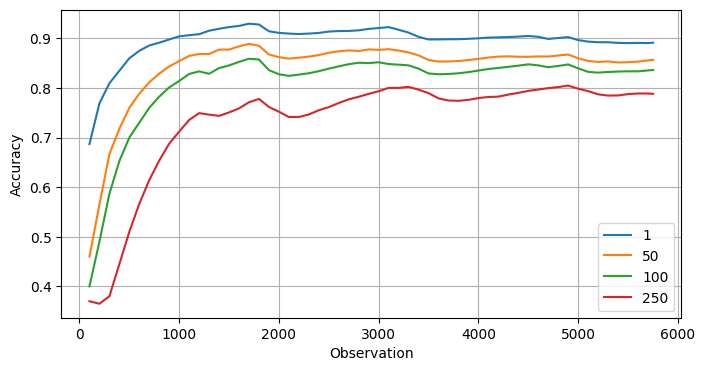
\includegraphics[width=\textwidth]{assets/design/gradual-learning-accuracy-delay-spectral-domain-fault.png}
        \caption{Spectral domain features}
    \end{subfigure}
    \caption{Incremental learning on all extracted feature with delayed reveal of labels in sliding windows.}
    \label{fig:design:online-fault-delay-sliding}
\end{figure}
	
	
The \textbf{tumbling window} simulates regular expert visits annotating observations recorded until that moment. Labels for the whole previous window are supplied at once. At the final sample, the accuracies are 83.41\% \emph{(temporal)} and 90.14\% \emph{(spectral)} with immediate feedback, and 77.95\% \emph{(temporal)} and 85.90\% \emph{(spectral)} with window length of 250 samples (Fig.~\ref{fig:design:online-fault-delay-tumbling}). 

\begin{figure}[ht]
    \centering
    \begin{subfigure}[b]{0.49\textwidth}
        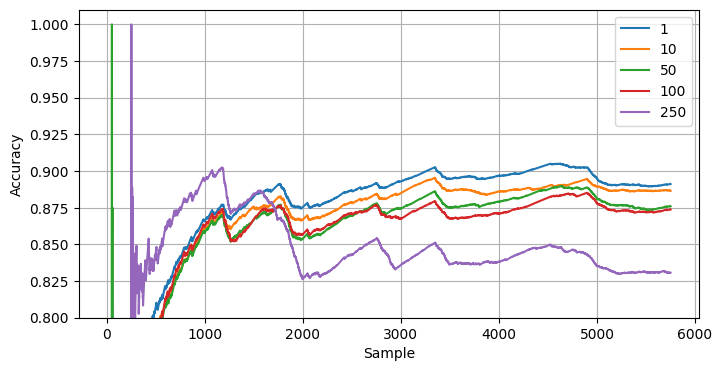
\includegraphics[width=\textwidth]{assets/design/gradual-learning-delay-temporal-domain-fault.png}
        \caption{Temporal domain features}
    \end{subfigure}
    \hfill
    \begin{subfigure}[b]{0.49\textwidth}
        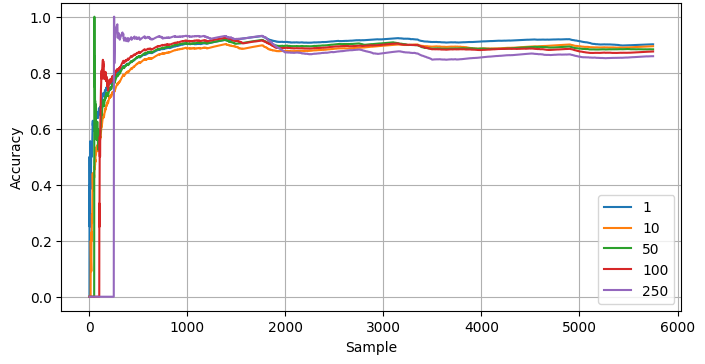
\includegraphics[width=\textwidth]{assets/design/gradual-learning-delay-spectral-domain-fault.png}
        \caption{Spectral domain features}
    \end{subfigure}
    \caption{Incremental learning on all extracted feature with delayed reveal of labels at regular intervals in tumbing windows.}
    \label{fig:design:online-fault-delay-tumbling}
\end{figure}

A \textbf{tumbling window} is more accurate according to progressive valuation because the labeling delay decreases towards the window's end. Initial 0\% accuracy is caused by a warming-up period in data collection during the span of the first few windows true labels are unknown. After just a handful of windows in the beginning, accuracy jumps above 60\% and stabilizes after 1000 observation.

Another common problem in online learning is \textbf{missing annotations} due to the size of the dataset. In the simulation of missing labels, the equal-length gaps are skipped before another observation is annotated. This approach of choosing samples to annotate without considering their representativeness results in severe harm to predictions. 

\begin{figure}[ht]
    \centering
    \begin{subfigure}[b]{0.49\textwidth}
        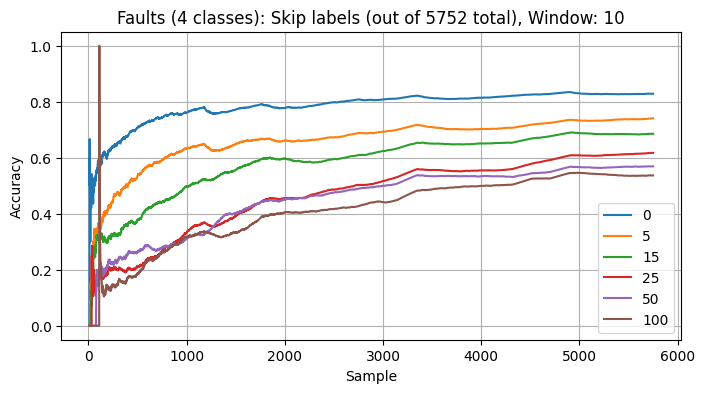
\includegraphics[width=\textwidth]{assets/design/gradual-learning-skip-temporal-domain-fault.png}
        \caption{Temporal domain features}
    \end{subfigure}
    \hfill
    \begin{subfigure}[b]{0.49\textwidth}
        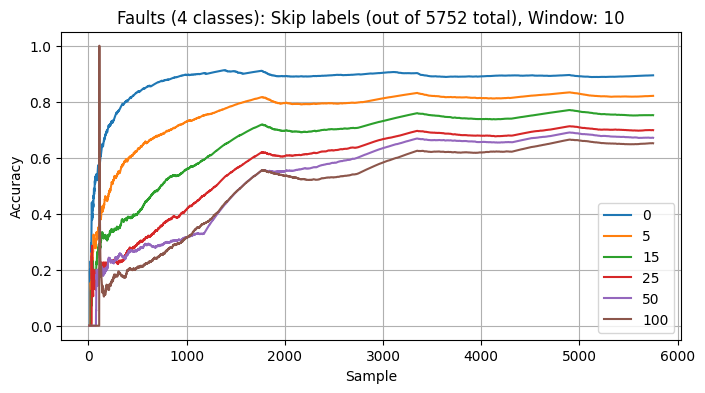
\includegraphics[width=\textwidth]{assets/design/gradual-learning-skip-spectral-domain-fault.png}
        \caption{Spectral domain features}
    \end{subfigure}
    \caption{Incremental learning with missing true labels and sliding window delay of 10 observations}
    \label{fig:design:online-label-skip}
\end{figure}

Labeling just every \nth{5} sample (25\% of the total dataset) with a sliding window delay of 10 samples reduces accuracy for the model out of temporal features by 8.77\% to 74.07\%, and by 7.33\% for spectral features to accuracy of 82.01\% (Fig.~\ref{fig:design:online-label-skip}). Even if only 1\% of the dataset is annotated (every \nth{100} sample), the model out of spectral features retained an accuracy of 65.17\%. The same cannot be said about the model from temporal features with very poor accuracy of 53.68\%. More missing labels require recording more observations before the equivalent accuracy is reached.


\section{Vibration measurement plan}

\subsection{Machinery}
% Enum list

\begin{figure}[ht]
    \centering
    \begin{subfigure}[b]{0.49\textwidth}
    		\centering
        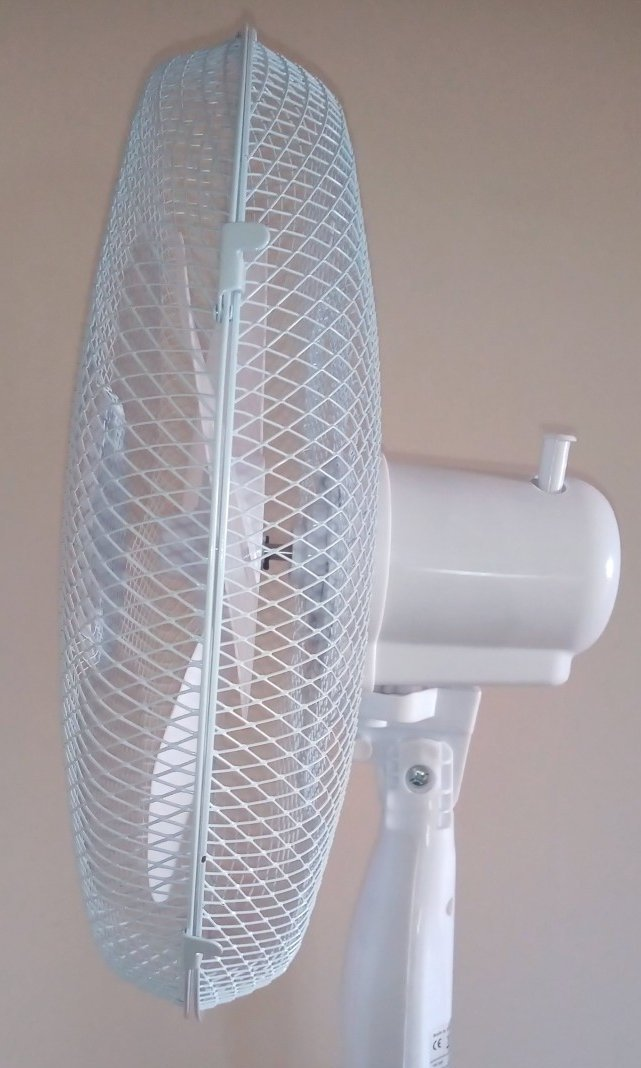
\includegraphics[width=0.5\textwidth]{assets/design/machine-fan.jpg}
        \caption{Stand fan Kalorik}
    \end{subfigure}
    \hfill
    \begin{subfigure}[b]{0.49\textwidth}
    		\centering
        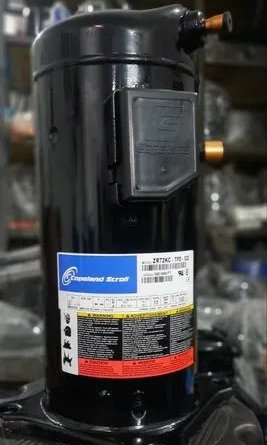
\includegraphics[width=0.5\textwidth]{assets/design/machine-compressor.jpg}
        \caption{Scroll compressor Copeland}
    \end{subfigure}
    \begin{subfigure}[b]{0.49\textwidth}
    		\centering
        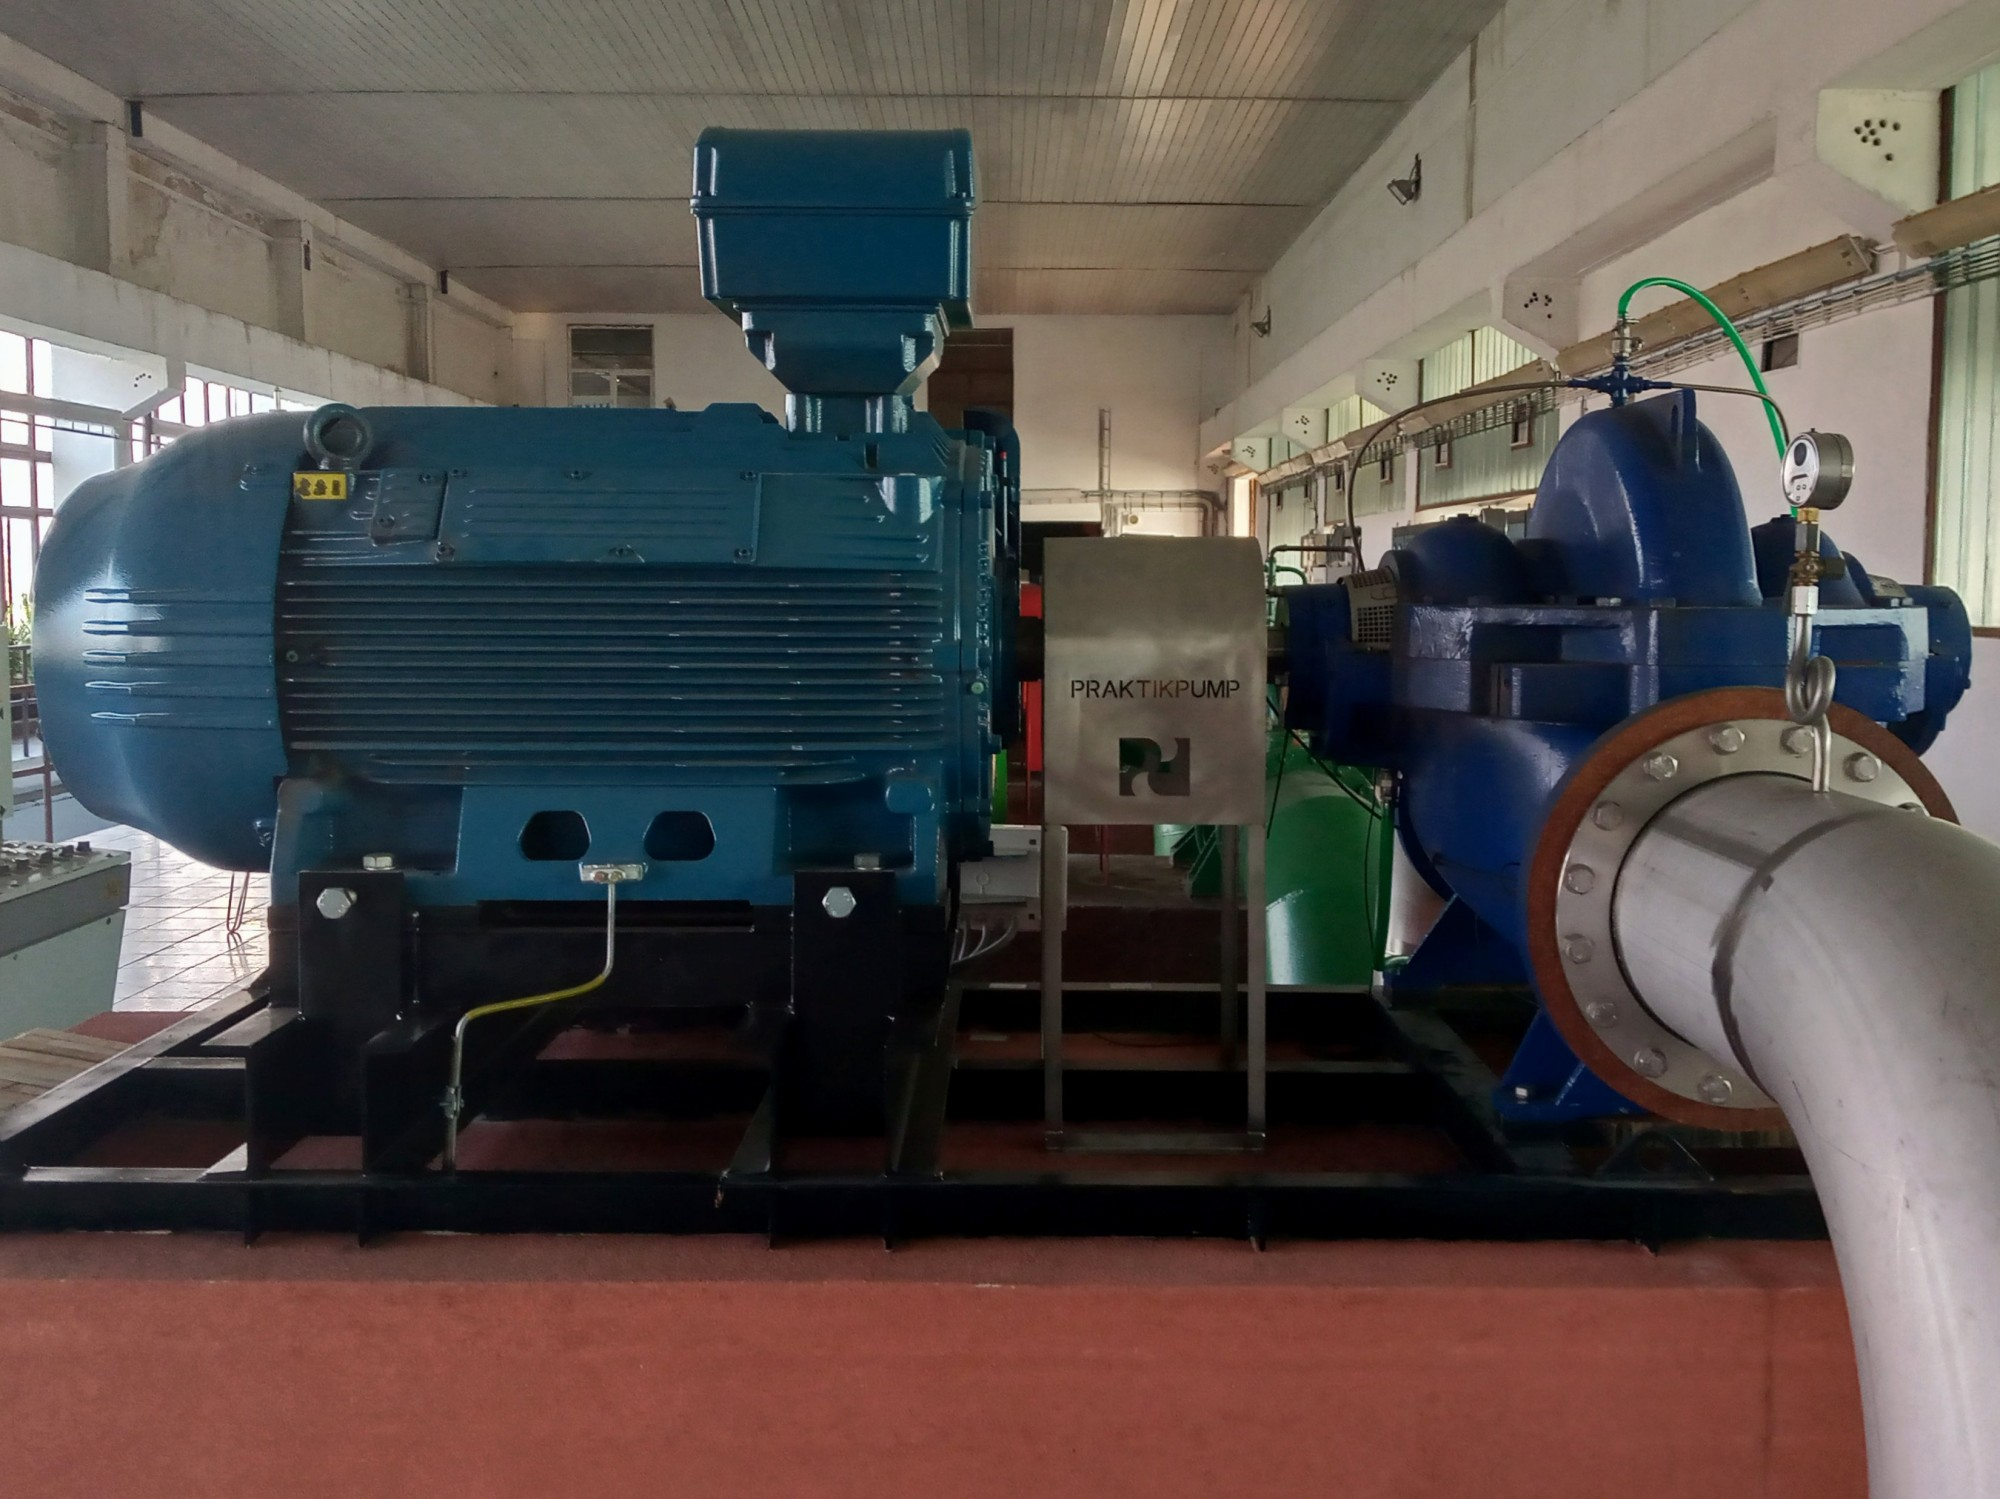
\includegraphics[width=\textwidth]{assets/design/machine-ksb-pump.jpg}
        \caption{Water pump KSB Omega}
    \end{subfigure}
    \hfill
    \begin{subfigure}[b]{0.49\textwidth}
    		\centering
        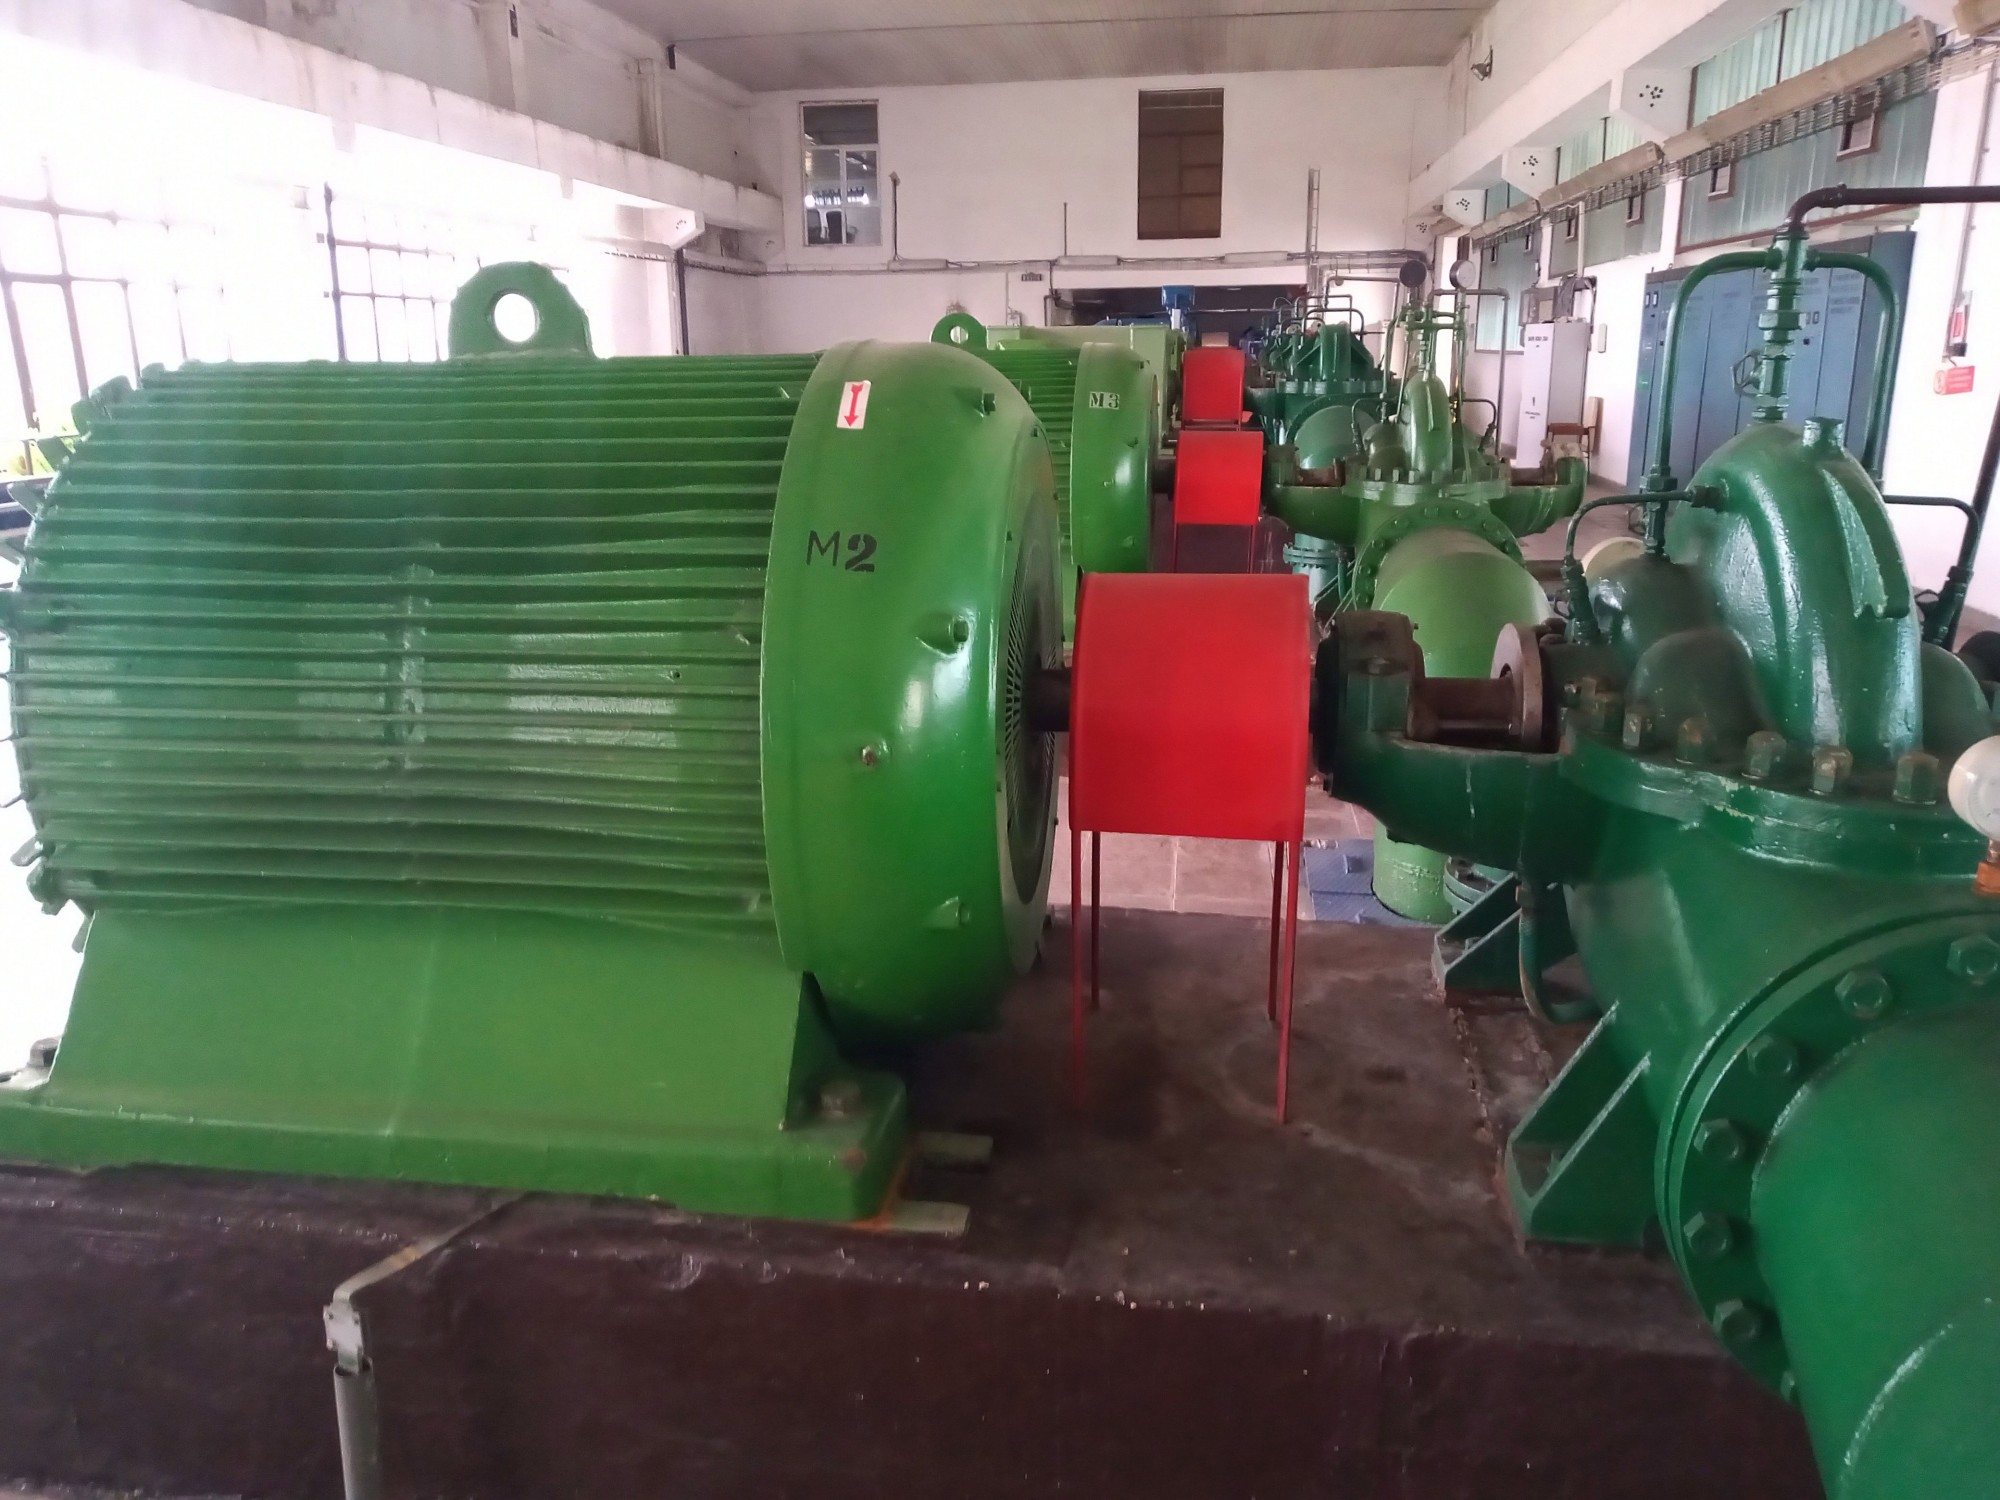
\includegraphics[width=\textwidth]{assets/design/machine-sigma-pump.jpg}
        \caption{Water pump Sigma}
    \end{subfigure}
    \caption{Machine}
\end{figure}


\subsection{Sensors}

\begin{table}[ht]
\renewcommand{\arraystretch}{1.2}
\centering
\begin{tabular}{|l|l|l|}
\hline
\textbf{Accelerometer}                           & \textbf{ADXL335} & \textbf{IIS3DWB}   \\ \hline
\textbf{Vendor}                                  & Analog Devices   & STMicroelectronics \\ \hline
\textbf{Bus}                                     & Analog           & SPI                \\ \hline
\textbf{Axis}                                    & 3                & 1 or 3             \\ \hline
\textbf{Range} (g)                               & $\pm$ 3          & $\pm$ 2 to 16      \\ \hline
\textbf{Bandwidth} (kHz)                         & 0.55             & 5 - 6.3            \\ \hline
\textbf{Sensitivity}                             & 300 mV/g         & 0.061 mg/LSB       \\ \hline
\textbf{Noise density} ($\mu g / \sqrt{\mathrm{Hz}}$ rms) & 150 - 300        & 75                 \\ \hline
\textbf{Microcontroller}                         & Beaglebone Black & ESP32-PoE-ISO      \\ \hline
\textbf{CPU SoC}                                 & TI Sitara AM3358 & ESP32-WROOM-32     \\ \hline
\textbf{Output data rate} (kHz)                  & 2.5              & 26.7               \\ \hline
\textbf{ADC resolution} (bit)                    & 12               & 16                 \\ \hline
\textbf{FIFO}                                    & -                & 3 kB (512 samples) \\ \hline
\end{tabular}
\caption{Accelerometers}
\end{table}


\begin{figure}[h]
	\centering
	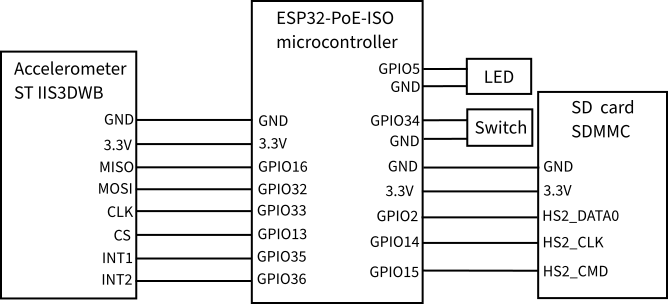
\includegraphics[width=\textwidth]{assets/design/hw-block-schematic.png}
	\caption{Sensor unit hardware block diagram}
\end{figure}

\subsection{Preliminary measurements}
\begin{figure}[ht]
    \centering
    \begin{subfigure}[b]{0.44\textwidth}
        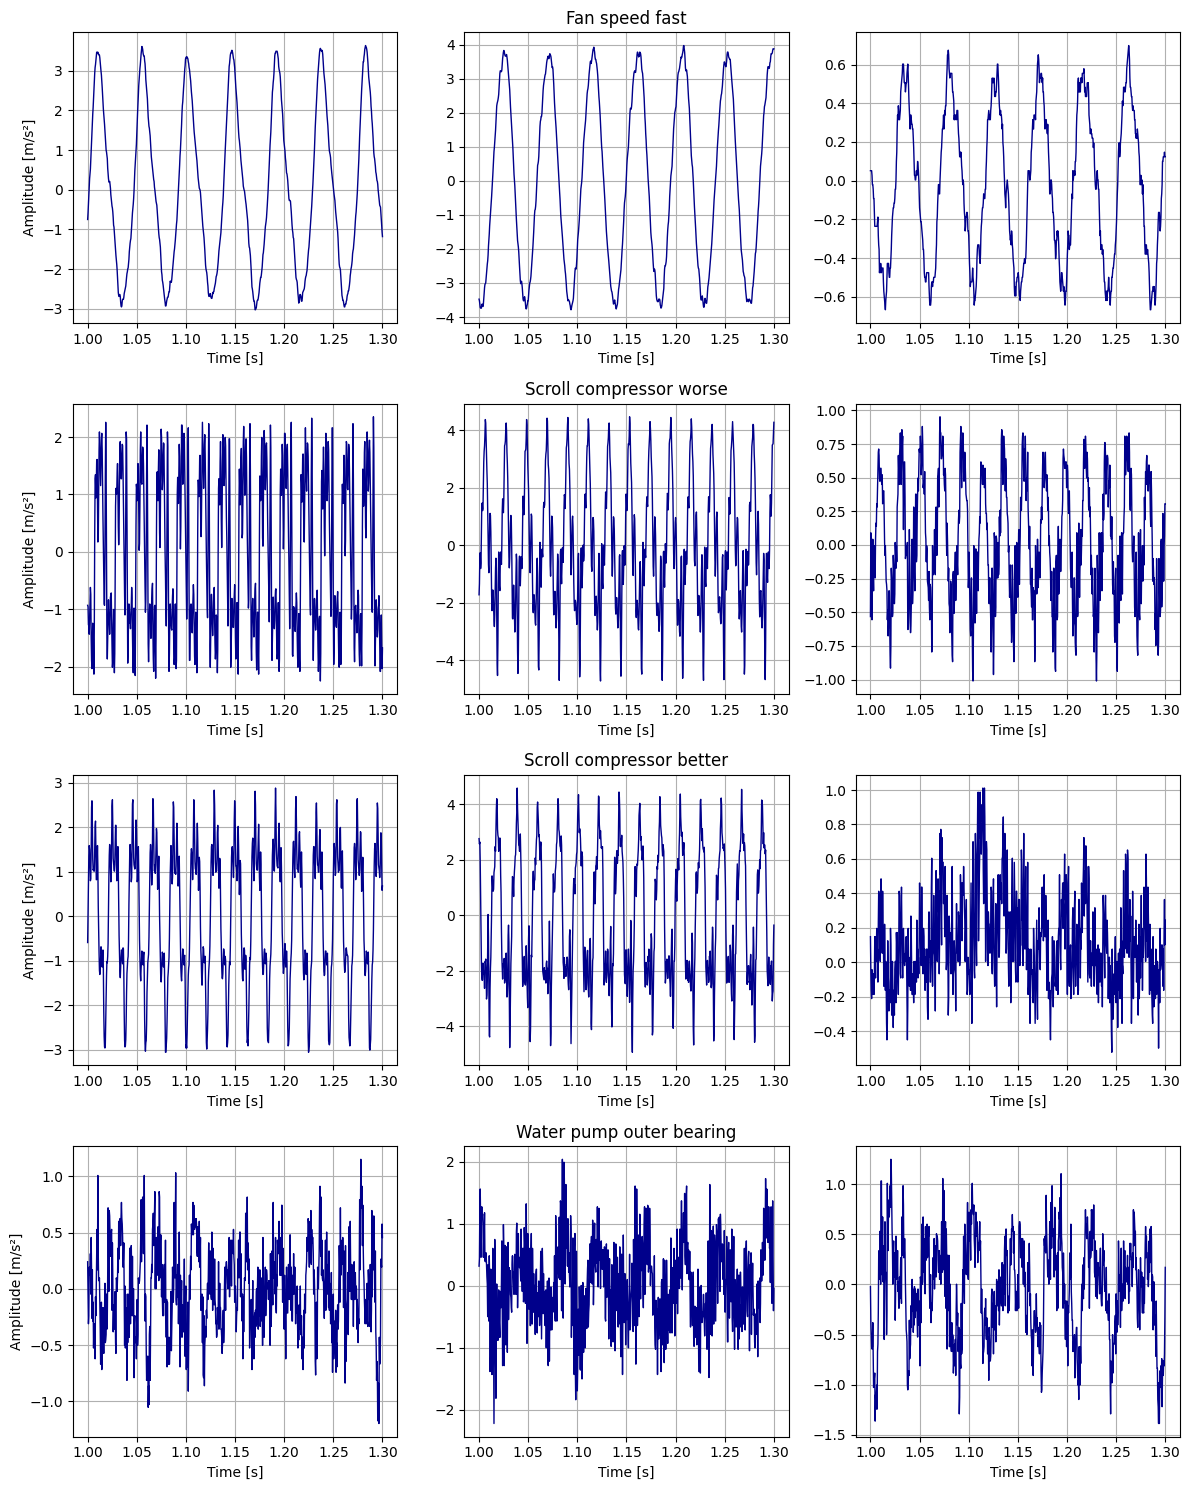
\includegraphics[width=\textwidth]{assets/design/EDA-custom-dataset-temporal.png}
        \caption{Temporal domain waveforms in all spatial directions with 300 ms duration}
    \end{subfigure}
    \hfill
    \begin{subfigure}[b]{0.55\textwidth}
        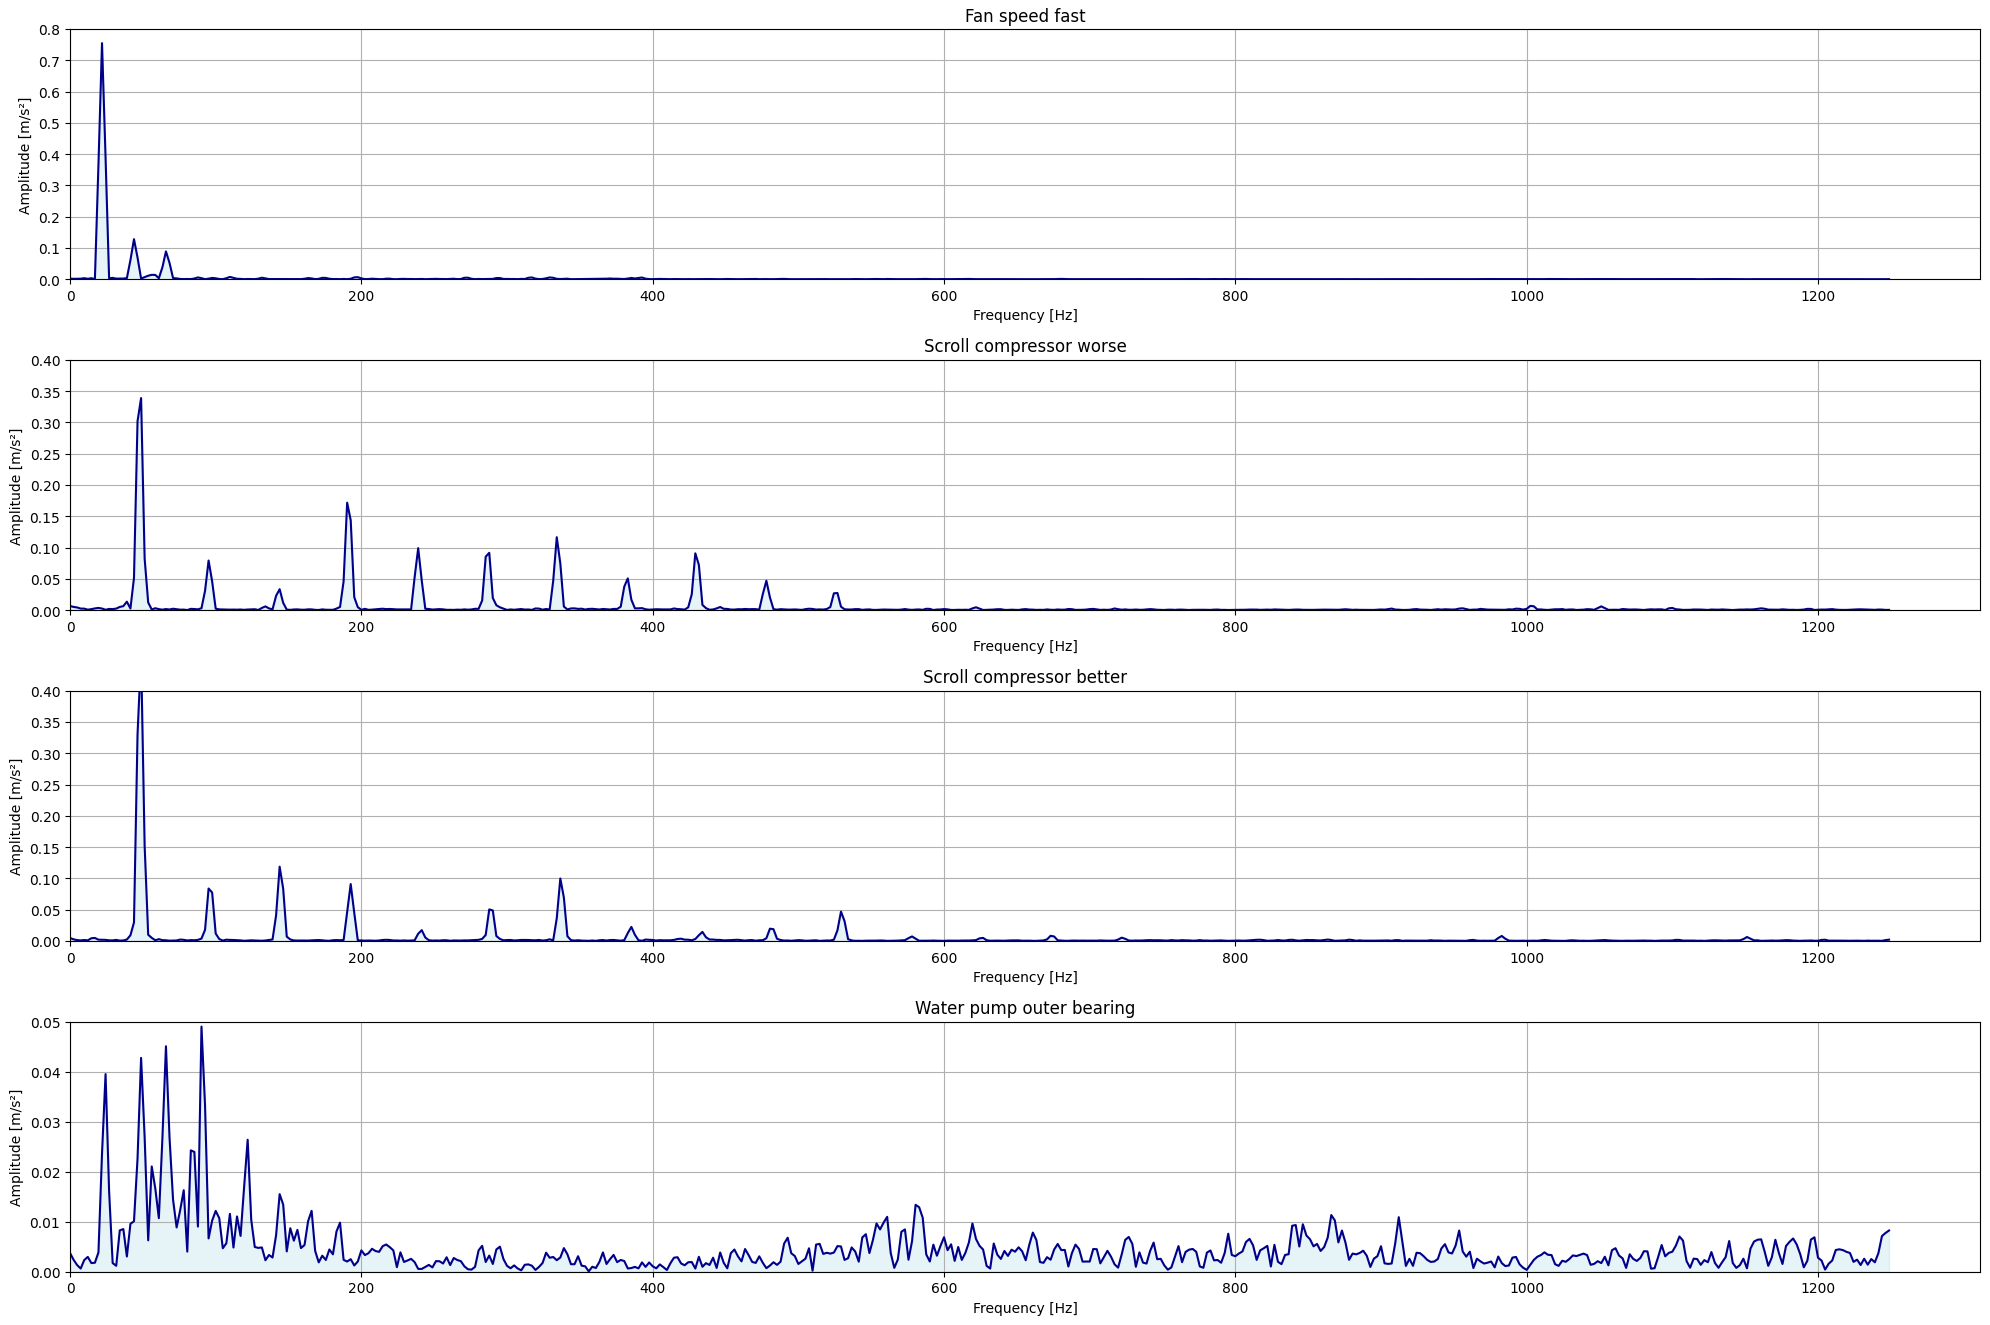
\includegraphics[width=\textwidth]{assets/design/EDA-custom-dataset-spectral-X-axis.png}
        \caption{Spectral domain in x accelerometer axis. FFT with Hann window of length $2^{10}$ ($\approx 409$ ms)}
    \end{subfigure} 
    \caption{Signals at 5 s timestamp}
\end{figure}


\begin{figure}[h]
	\centering
	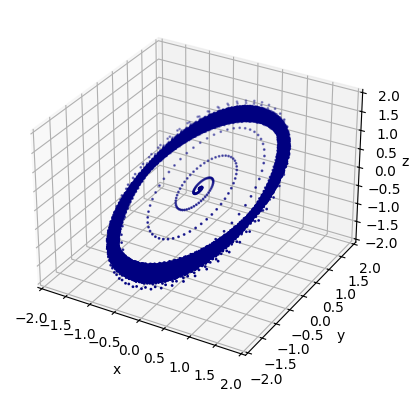
\includegraphics[width=0.6\textwidth]{assets/design/compressor-orbitals-1x.png}
	\caption{Orbital analysis of compressor's 1x harmonic}
\end{figure}

